% This work is licensed under the Creative Commons
% Attribution-NonCommercial-ShareAlike 3.0 Unported License. To view a copy of
% this license, visit http://creativecommons.org/licenses/by-nc-sa/3.0/ or send
% a letter to Creative Commons, 444 Castro Street, Suite 900, Mountain View,
% California, 94041, USA.

\documentclass{mycourse}

\usepackage{xfrac}
\ExplSyntaxOn
\DeclareCollectionInstance{plainmath}{xfrac}{mathdefault}{math}
{
denominator-bot-sep = 0 pt,
numerator-bot-sep = 2 pt,
numerator-top-sep = \c_max_dim,
scaling = true,
scale-factor = 0.5,
h-scale = 0.7,
v-scale = 0.8,
slash-right-mkern = -3 mu,
slash-left-mkern = -3 mu,
}
\UseCollection{xfrac}{plainmath}
\ExplSyntaxOff

\usepackage{braket}

\usetikzlibrary{arrows,positioning}
\usepackage{tikz-cd}
\tikzset{
	commutative diagrams/sur/.style={two heads},
	commutative diagrams/inj/.style={hook},
	commutative diagrams/bij/.style={inj, sur},
	commutative diagrams/hom/.style={bij},
}

\newcommand{\B}{\mathbb{B}}
\newcommand{\D}{\mathbb{D}}
\renewcommand{\S}{\mathbb{S}}
\newcommand{\boundary}{\delta}
\newcommand{\dunion}{\sqcup}
\newcommand{\bigdunion}{\bigsqcup}
\newcommand{\oBdA}{o.B.d.A.}
\newcommand{\coursehref}[2]{\href{http://www.igt.uni-stuttgart.de/eiserm/lehre/2013/Topologie/Arbeitsblaetter/#1}{#2}}
\newcommand{\injto}{\hookrightarrow}
\newcommand{\surto}{\to}
\newcommand{\bijto}{\xrightarrow{\sim}}
\newcommand{\homeomorphic}{\cong}
\newcommand{\homto}{\xrightarrow{\raisebox{-2pt}[0pt][0pt]{\ensuremath{\scriptstyle{\homeomorphic}}}}}
\newcommand{\eqq}{\equiv}
\newcommand{\homotopic}{\simeq}


\NewDocumentCommand \SepAxiom { m } { \ensuremath{\mathrm{T_{#1}}} }
\DeclareDocumentCommand \Cat { m } { \underline{\mathrm{#1}} }
\DeclareDocumentCommand \Ob { } { \mathrm{Ob} }
\DeclareDocumentCommand \Mor { } { \operatorname{Mor} }
\DeclareDocumentCommand \Vec { } { \operatorname{Vec} }
\DeclareDocumentCommand \isomorphic { } { \cong }
\DeclareDocumentCommand \isoto { } { \xrightarrow{\isomorphic} }


%% no numbering
%\makeatletter
%\renewtheoremstyle{mythm}%
%	{\item[\rlap{\vbox{\hbox{\hskip\labelsep \theorem@headerfont
%			{\color{theoremtype}##1}\ \theorem@separator}\hbox{\strut}}}]}%
%	{\item[\rlap{\vbox{\hbox{\hskip\labelsep \theorem@headerfont
%			{\color{theoremtype}##1}\ \color{theoremtitle}(##3)\theorem@separator}\hbox{\strut}}}]}
%\makeatother

\renewtheorem{thm}{Theorem}[section]
\renewcommand{\thechapter}{\Alph{chapter}}
\renewcommand{\thesection}{\thechapter\relax\arabic{section}}


\begin{document}

\title{Topologie}

\maketitle

\tableofcontents

% Alphabetical
\chapter{Was ist und was soll die Topologie?}

\coursetimestamp{14}{10}{2013}

Dieser Frage wollen wir natürlich im Laufe der gesamten Vorlesung auf den Grund gehen.
Deshalb zunächst eine vorläufige Antwort: Topologie ist qualitative Geometrie.

\emph{Homöomorphie} gehört zu den Begriffen, mit denen die Topologie qualitative Aussagen über die Geometrie verschiedener Räume macht.

\begin{ex}
	% fixme: images
	Ränder von Dreiecken, Quadraten und Kreisen sind \emph{homöomorph}.
	Flächen von Dreiecken, Quadraten und Kreisen sind \emph{homöomorph}.
	Die Ränder sind jedoch nicht zu den Flächen homöomorph.
\end{ex}


\section{Zentrales Beispiel: Flächen}


% fixme: img: sphere, torus, …

\begin{df}
	Eine (berandete) \emph{Fläche} ist ein metrischer Raum, der lokal homöomorph ist zu
	\[
		\R^2_+ := \{ (x,y) \in \R^2 \suchthat x \ge 0 \}
	\]
\end{df}

\begin{ex}
	Zu $g \in \N, r \in \N_{\ge 1}$ betrachten wir
	\begin{align*}
		F_{g,r}^+ := % fixme: img
		F_{g,r}^- := % fixme: img
	\end{align*}
	% fixme: img: F_{0,1}^+, F_{0,2}^+, F_{0,1}^-

	% fixme: Definition für r=0
	Flächen ohne Rand: $F_g^+ := F_{g,0}^+$, $F_g^- := F_g^+ / \{\pm 1\}$.

	Diese Beispiele $F_{g,r}^{\pm}$ sind kompakte und zusammenhängende Flächen.

	Es stellen sich folgende Fragen
	\begin{enumerate}[1)]
		\item
			Ist unsere Liste vollständig?
		\item
			Ist unsere Liste redundanzfrei?
	\end{enumerate}
\end{ex}

\begin{ex}
	% fixme: img
	Sind diese Beispiele homöomorph zu $F_{g,r}^{\pm}$?
\end{ex}

\begin{st}[Klassifikation der kompakten Flächen]
	Jede kompakte, zusammenhängende Fläche $F$ ist homöomorph zu genau einem der Modelle $F_{g,r}^\pm$.
\end{st}

Wir werden in dieser Vorlesung wie folgt vorgehen:

\begin{enumerate}[1.]
	\item
		Analytische Topologie
	\item
		Geometrische Topologie
	\item
		Algebraische Topologie
\end{enumerate}

\chapter{Metrische Räume}

% paragraph B1
\section{Reelle Zahlen}

\begin{st}[Existenz und Eindeutigkeit der reellen Zahlen]
	Es existiert ein vollständiger, geordneter Körper $(\R,+,\cdot,<)$.

	Je zwei solcher Körper sind isomorph mittels eines eindeutig bestimmten Körperhomomorphismus.
\end{st}


\section{Skalarprodukt und Norm}

\begin{df}
	Sei $\K \in \{\R, \C\}$.
	Auf $V := \K^n$ definieren wir das \emph{Skalarprodukt}
	\[
		\<\argdot, \argdot\> : V \times V \to \K
	\]
	durch
	\[
		\<(x_1,\dotsc, x_n), (y_1,\dotsc, y_n)\> := \_{x_1}y_1 + \dotsb + \_{x_n}y_n.
	\]
	Es gelten
	\begin{enumerate}[({S}1),start=0]
		\item
			$\<x,x\>  \in \R_{\ge 0}$,
		\item
			$\<x,x\> > 0$ für $x \neq 0$,
		\item
			$\<y,x\> = \_{\<x,y\>}$,
		\item
			$\<x,\lambda y + \my z\> = \lambda \<x,y\> + \my\<x,z\>$.
	\end{enumerate}
	Jede Abbildung $V\times V \to \K$ mit (S0-3) ist ein Skalarprodukt.
\end{df}

\begin{ex}
	Sei $\Omega$ eine Menge, $\K^{\Omega} := \{f : \Omega \to \K\}$,
	\[
		\K^{(\Omega)} = \{ f: \Omega \to \K : f \text{ hat endlichen Träger} \}.
	\]
	Dann ist
	\[
		\<f,g\> := \sum_{x\in \Omega} \_{f(x)}g(x)
	\]
	ein Skalarprodukt
\end{ex}

\begin{ex}
	Auf $V = C([a,b], \C)$ ist
	\[
		\<f,g\> = \f 1{b-a} \int_{x-a}^b \_{f(x)} g(x) \dx
	\]
	ein Skalarprodukt.
\end{ex}

\begin{st}
	Sei $V$ ein $K$-Vektorraum und $\<\argdot, \argdot\>$ ein Skalarprodukt.
	Dann gilt die Cauchy-Schwartz-Ungleichung (CSU):
	\[
		|\<u,v\>|^2 \le \<u,u\> \<v,v\>.
	\]
	Hieraus folgt für die Norm $|u| := \sqrt{\<u,u\>}$
	\begin{enumerate}[({N}1),start=0]
		\item
			$|0| = 0$
		\item
			$|v| > 0$ für  $v\neq 0$
		\item
			$|\lambda v| = |\lambda| |v|$ für $v \in V, \lambda \in K$.
		\item
			$|u+v| \le |u| + |v|$ (Dreiecksungleichung)
	\end{enumerate}
\end{st}

\begin{df}
	Eine \emph{Norm} auf $V$ ist eine Abbildung $|\argdot| : V \to \R_{\ge 0}$, die (N0-3) erfüllt.
\end{df}

\begin{ex}
	Auf $\R^n$:
	\begin{itemize}
		\item
			\emph{Taxinorm} oder $\ell^1$-Norm:
			\[
				|x|_1 = |x_1| + \dotsb + |x_n|.
			\]
		\item
			\emph{Euklidische Norm} oder $\ell^2$-Norm:
			\[
				|x|_2 = \sqrt{|x_1|^2 + \dotsb + |x_n|^2}.
			\]
		\item
			\emph{Supremumsnorm} oder $\ell^\infty$-Norm:
			\[
				|x|_\infty := \sup \{ |x_1|, \dotsc, |x_n| \}
			\]
		\item
			Allgemeine $\ell^p$-Norm ($1\le p < \infty$):
			\[
				|x|_p := \Big( |x_1|^p + \dotsb + |x_n|^p \Big)^{\f 1p}
			\]
			% fixme: Skizze zu $B_p := \{x\in \R^2 : |x|_p \le 1\}$
	\end{itemize}
	\begin{note}
		Auf $\R^n$ gilt
		\[
			|x|_\infty
			\le |x|_2
			\le |x|_1
			\le n |x|_\infty
		\]
	\end{note}
\end{ex}

\begin{ex}
	Sei $\K = \R, \C$ und $\Omega$ ein Menge.
	Wir schreiben
	\begin{align*}
		\Abb(\Omega, \K) = \K^\Omega &:= \{f : \Omega \to \K\} \\
		\|f\|_{\infty} := |f|_\Omega &:= \sup \{ |f(x)| : x \in \Omega \} \\
		\|f\|_{p} &:= \bigg( \sum_{x\in\Omega} |f(x)|^p \bigg)^{\f 1p} \\
		\ell^p(\Omega) &:= \{ f : \Omega \to \K : \|f\|_p < \infty \}
	\end{align*}
\end{ex}

\begin{ex}
	Sei $\Omega \subset \R^n$ messbar, $f : \Omega \to \R$ messbar,
	\begin{align*}
		\|f\|_p &:= \bigg( \int_{x\in \Omega} |f(x)|^p \dx \bigg)^{\f 1p} \\
		\scr L^p(\Omega) &:= \{ f: \Omega \to \K : \|f\|_p < \infty \}
	\end{align*}
	Aus $\|f\|_p = 0$ folgt nur $f=0$ fast überall.
	Setze
	\begin{align*}
		N &:= \{ f : \Omega \to \K : f(x) = 0 \text{ für fast alle $x\in\Omega$} \\
		L^p &:= \ell^p / N
	\end{align*}
	Auf $L^p(\Omega)$ ist $\|\argdot\|_p$ tatsächlich eine Norm.
\end{ex}

\begin{ex}
	Für Matrizen $A \in \K^{m\times n}$ setze
	\[
		|A| := \bigg( \sum_{i=1}^m \sum_{j=1}^n |a_{ij}|^2 \bigg)^{\f 12}.
	\]
	Dies ist ein Norm (Euklidische Norm auf $\K^{mn}$) und erfüllt zudem
	\[
		|A B | \le |A| |B|,
		\qquad A \in \K^{m\times n}, \B \in \K^{n\times m}.
	\]
	Insbesondere $|Av| \le |A| |v|$ für $v\in \K^n (= \K^{n\times 1})$.
\end{ex}

\begin{ex}
	$\K^{n\times n}$ ist eine Algebra über $\K$ mit Norm $|A|$ wie oben.
\end{ex}

\begin{df}
	Eine \emph{normierte $\K$-Algebra} ist eine Algebra $(A_i)$ über $\K$ mit einer Norm $|\argdot|: A \to \R_{\ge 0}$, sodass $|uv| \le |u||v|$ für alle $u,v \in A$ gilt.
\end{df}

\begin{ex}
	Sei $\K = \R, \C$.
	Beispiele für normierte Algebren sind
	\begin{itemize}
		\item
			$\K^{n\times n}$
		\item
			$\ell^\infty(\Omega, \K)$
	\end{itemize}
\end{ex}


\section{Metrische Räume}


\begin{ex}
	Betrachte den Euklidischen Abstand auf $\R^n$
	\[
		d(x,y) = |x-y|_2 = \sqrt{ (x_1 - y_2)^2  + \dotsb + (x_n - y_n)^2 }.
	\]
	Es gelten folgende Eigenschaften
	\begin{enumerate}[({M}1),start=0]
		\item
			$d(x,x) = 0$
		\item
			$d(x,y) > 0$ für $x\neq y$
		\item
			$d(x,y) = d(y,x)$
		\item
			$d(x,z) \le d(x,y) + d(y,z)$
	\end{enumerate}
\end{ex}

\begin{df}
	Sei $X$ eine Menge.
	Eine \emph{Metrik} auf $X$ ist eine Abbildung $d : X \times X \to [0, \infty]$, die (M0-3) erfüllt.

	Das Paar $(X,d)$ heißt dann \emph{metrischer Raum}.
\end{df}

\begin{ex}
	$X = \R^n$ mit $d$ der euklidischen Metrik.
\end{ex}

\begin{ex} \label{ex:discrete_metric}
	Auf jeder Menge $X$ haben wir die \emph{diskrete Metrik}
	\[
		d(x,y) = \begin{cases}
			0 & x=y \\
			1 & x\neq y
		\end{cases}.
	\]
\end{ex}

\begin{df}
	Ein metrischer Raum mit der diskreten Metrik aus \ref{ex:discrete_metric}
	\[
		d(x,y) = \begin{cases}
			0 & x=y \\
			1 & x\neq y
		\end{cases}
	\]
	nennen wir \emph{diskreter metrischer Raum}.
\end{df}

\begin{ex}
	Die \emph{französische Eisenbahnmetrik} $d: \R^n \times \R^n \to \R_{\ge 0}$
	\[
		d(x,y) := \begin{cases}
			|x-y|_2 & \R x = \R y \\
			|x|_2 + |y|_2 & \R x \neq \R y
		\end{cases}
	\]
\end{ex}

\begin{ex}[Teilräume]
	Ist $(X,d)$ ein metrischer Raum und $A \subset X$, dann ist $d_A := d\big|_{A\times A} : A \times A \to [0,\infty]$ eine Metrik auf $A$.
\end{ex}

\begin{ex}[Produkträume]
	Seien $(X,d_i)$ mit $i \in I$ metrische Räume.
	Auf $X = \prod_{i\in I} X_i$ (dem Produktraum) erhalten wir die Supremumsmetrik
	\[
		d(x,y) := \sup \{ d_i(x_i,y_i) : i \in I \}.
	\]
\end{ex}

\begin{ex}[Abbildungsräume]
	Ist $(Y,d_y)$ ein metrischer Raum, $X$ eine Menge, dann trägt $Y^X = \Abb(X,Y)$ die Metrik
	\[
		d(f,g) := \sup \{ d_y(f(x),g(x)) : x \in X \}
	\]
	für $f,g : X \to Y$.
\end{ex}

\begin{df}
	Eine \emph{isometrische Einbettung} $f:(X,d_X) \to (Y,d_Y)$ ist eine Abbildung $f: X\to Y$ mit $d(f(a), f(b)) = d_X(a,b)$ für alle $a,b \in X$.
	Ist $f$ bijektiv, so heißt $f$ eine \emph{Isometrie}.
\end{df}

\begin{ex}
	Verschiebungen, Drehungen, Spiegelungen auf $\R^n$.
\end{ex}

\begin{ex}
	Sei $m \le n$, dann ist	$f: \R^n \to \R^n$ mit
	\[
		f(x_1, \dotsc, x_m) = (x_1, \dotsc, x_m, 0, \dotsc, 0)^T
	\]
	eine isometrischen Einbettung.
\end{ex}

\begin{ex}
	Die Räume $\ell^2(\Z, \C)$ und $L^2([0,2\pi], \C)$ sind isometrisch dank Fourier-Analyse/Synthese.
\end{ex}

Seien $(X,d_X), (Y,d_Y)$ metrische Räume.
Jede Funktion $f : X \to Y$ erfüllt
\[
	l d(a,b) \le d(f(a), f(b)) \le L d(a,b)
\]
für alle $a,b \in X$ mit den Konstanten $l=0, L = \infty$.

\begin{df}
	Wir nennen $f$ \emph{Lipschitz-stetig} wenn
	\[
		l \cdot d(a,b) \le d(f(a), f(b)) \le L \cdot d(a,b)
	\]
	für ein $L$ mit $0 \le L < \infty$ gilt.

	Ist zusätzlich $0 < l \le L < \infty$, so heißt $f$ \emph{bi-Lipschitz-stetig}.
\end{df}

\begin{ex}
	\begin{itemize}
		\item
			$f$ ist Isometrie genau dann, wenn $l=L=1$ genügt.
		\item
			$f$ ist konstant genau dann, wenn $L=0$ genügt.
	\end{itemize}
\end{ex}

\begin{ex}
	\begin{itemize}
		\item
			$f(x) = x^2$, $L=2, l=0$.
		\item
			$g(x) = \sqrt{x}$, $L=\infty, l=\f 12$.
	\end{itemize}
\end{ex}

\begin{df}
	In einem metrischen Raum $(X,d)$ ist der \emph{offene Ball} um $a \in X$ mit Radius $r\in [0,\infty]$ die Menge
	\[
		B(a,r) := B_{(X,d)}(a, r) := \{ x \in X : d(a,x) < r \}.
	\]
	Der \emph{abgeschlossene Ball} ist
	\[
		\_{B}(a,r) := \_{B}_{(X,d)}(a, r) := \{ x \in X : d(a,x) \le r \}.
	\]
\end{df}

\begin{df}
	Eine Menge $U \subset X$ heißt \emph{Umgebung} von $a$ in $(X,d)$, wenn es $\eps \in \R_{> 0}$ gibt, sodass $B(a,\eps) \subset U$.

	Die Menge $U$ heißt \emph{offen} in $(X,d)$, wenn sie Umgebung jedes Punktes $a \in U$ ist.

	Eine Menge $A \subset X$ heißt \emph{abgeschlossen} in $(X,d)$, wenn $X \setminus A$ offen ist in $(X,d)$.

	Die Familie $\_{S_{X,d}}$ aller offenen Mengen heißt die \emph{Topologie} des Raumes $(X,d)$.
\end{df}

\begin{prop}
	Jeder offene Ball ist offen.
	Jeder abgeschlossene Ball ist abgeschlossen.

	Es gelten
	\begin{enumerate}[({O}1)]
		\item
			$\emptyset, X$ sind offen.
		\item
			$U_1,\dotsc,U_n$ offen $\implies U_1 \cap \dotsb \cap U_n$ offen.
		\item
			$U_i$ offen ($i\in I$) $\implies \bigcup_{i\in I} U_i$ offen.
	\end{enumerate}
	\begin{enumerate}[({A}1)]
		\item
			$\emptyset, X$ sind abgeschlossen.
		\item
			$A_1,\dotsc,A_n$ abgeschlossen $\implies A_1 \cup \dotsb \cup A_n$ offen.
		\item
			$A_i$ abgeschlossen ($i\in I$) $\implies \bigcap_{i\in I} A_i$ offen.
	\end{enumerate}
\end{prop}

\begin{df}
	Zu $M \subset X$ definieren wir das \emph{Innere} von $M$ in $(X,d)$ durch
	\begin{align*}
		\mathring M &:= \{ x \in X : M \text{ ist Umgebung von $x$ in $(X,d)$} \} \\
		&= \{ x \in X : \exists \eps > 0 B(x,\eps) \subset M \} \\
		&= \bigcup \{ U \subset M : U \text{ ist offen in $(X,d)$}.
		% fixme: prüfen
	\end{align*}

	Der \emph{Abschluss} (oder abgeschlossene Hülle) von $M$ in $(X,d)$ ist
	\begin{align*}
		\_{M} &:= \{ x \in X : \text{ Jede Umgebung von $x$ in $(X,d)$ schneidet $M$} \} \\
		&= \{ x \in X : \forall \eps > 0 : B(x,\eps) \cap M \neq \emptyset \} \\
		&= \bigcap \{ A \supset M : \text{$A$ ist abgschlossen in $(X,d)$} \}
		% fixme: prüfen
	\end{align*}

	Der \emph{Rand} $\boundary M$ von $M$ in $(X,d)$ ist
	\[
		\boundary M := \_{M} \setminus \mathring M
	\]
\end{df}

\begin{ex}
	Im $\R^n$ betrachten wir
	\begin{align*}
		\D^n := \{ x \in \R^n : x_1^2 + \dotsb + x_n^2 \le 1 \}, \\
		\B^n := \{ x \in \R^n : x_1^2 + \dotsb + x_n^2 < 1 \}, \\
		\S^{n-1} := \{ x \in \R^n : x_1^2 + \dotsb + x_n^2 = 1 \}.
	\end{align*}
\end{ex}

\coursetimestamp{21}{10}{2013}

\begin{nt}
	Wir verwenden für ein Mengensystem $\scr A$ die Notation für die Vereinigung über alle enthaltenen Mengen
	\[
		\bigcup \scr A
		= \bigcup_{A \in \scr A}
		= \bigcup_{i\in I} A_i.
	\]
\end{nt}


\section{Konvergenz und Stetigkeit}

Sei im Folgenden $(X,d)$ stets ein metrischer Raum.

\begin{df}
	Eine Folge $(x_n)_{n\in \N}$ in $X$ \emph{konvergiert} gegen $a \in X$, wenn $d(x_n, a) \to 0$, d.h.
	\[
		\forall \eps > 0 \exists m \in \N \forall n \ge m : d(x_n, a) < \eps,
	\]
	oder mit anderen Worten: Jede Umgebung von $a$ enthält fast alle Folgenglieder.
\end{df}

\begin{df}
	Eine Funktion $f: X \to Y$ heißt stetig in einem Punkt $a \in X$, wenn
	\[
		\forall \eps > 0 \exists \delta > 0 : \forall x \in X : d_X(x,a) < \delta \implies d_Y(f(x), f(a)) < \eps.
	\]

	Die Funktion $f: X \to Y$ heißt \emph{stetig} (auf ganz $X$), wenn
	\[
		\forall a \in X \forall \eps > 0 \exists \delta > 0 \forall x \in X: d_X(x,a) < \delta \implies d_Y(f(x), f(a)) < \eps
	\]
	und \emph{gleichmäßig stetig}, wenn
	\[
		\forall \eps > 0 \exists \delta > 0 \forall x,a \in X: d_X(x,a) < \delta \implies d_Y(f(x), f(a)) < \eps
	\]

	Die Menge aller stetigen Abbildung $f: X \to Y$ bezeichnen wir mit $C(X,Y)$.

	Ist $f$ bijektiv und sowohl $f$, als auch $f^{-1}$ stetig, so heißt $f$ \emph{Homöomorphismus}.
\end{df}

\begin{st}
	Für $f: X \to Y$ sind äquivalent
	\begin{enumerate}[1)]
		\item
			$f$ ist stetig,
		\item
			$f$ ist folgenstetig, d.h. aus $x_n \to a$ in $X$ folgt $f(x_n) \to f(a)$ in $Y$,
		\item
			Für $V \subset Y$ offen ist $f^{-1}(V) \subset X$ offen,
		\item
			Für $V \subset Y$ abgeschlossen ist $f^{-1}(V) \subset X$ abgeschlossen.
	\end{enumerate}
	\begin{proof}
		Übungsaufgabe % fixme: reference
	\end{proof}
\end{st}

\begin{df}
	Eine Folge $f_n: X \to Y$ \emph{konvergiert punktweise} gegen $f: X \to Y$, wenn für alle $x \in X$ gilt $f_n(x) \to f(x)$, d.h.
	\[
		\forall x \in X \forall \eps > 0 \exists m \in \N \forall n \ge m : d_Y(f_n(x), f(x)) \le \eps.
	\]
	Hingegen konvergiert $f_n: X \to Y$ \emph{gleichmäßig} gegen $f: X \to Y$, wenn
	\[
		\forall \eps > 0 \exists m \in \N \forall n \ge m \underbrace{\forall x \in X : d_Y(f_n(x), f(x)) \le \eps}_{\iff d (f_n, f) \le \eps},
	\]
	wobei
	\[
		d(f,g)
		:= \sup \{ d_Y(f(x), g(x)) : x \in X \}.
	\]
\end{df}

\begin{ex}
	Sei $f_n : [0,1] \to \R, f_n(x) := x^n$.
	Dann konvergiert $(f_n)$ punktweise gegen $f:[0,1] \to \R$ mit $f(x) = 0$ für $0 \le x < 1$ und $f(x) = 1$ für $x=1$.

	Die Konvergenz ist nicht gleichmäßig, denn
	\[
		|f_n - f|_{[0,1]} = 1
	\]
\end{ex}

\begin{ex}
	Die Polynome $f_n(x) = \sum_{k=0}^n \f{(-1)^k}{2k!} x^{2k}$ konvergieren in jedem $x \in \R$ gegen $f(x) = \cos(x)$.

	Die Konvergenz ist jedoch nicht gleichmäßig, denn es gilt
	\[
		|f_n - f|_{\R} = \infty.
	\]
	Wir haben aber immerhin gleichmäßige Konvergenz auf jedem Kompaktum $[-r,r] \subset \R$.
\end{ex}

\begin{st}
	Konvergiert $f_n \to f$ gleichmäßig und sind alle $f_n$ stetig, so auch $f$.
	\begin{proof}
		Übungsaufgabe % fixme: reference
	\end{proof}
\end{st}

\begin{st}[Zwischenwertsatz]
	Jede stetige Funktion $f: [a,b] \to \R$ hat die Zwischenwerteigenschaft (ZWE): zu $y \in \R$ mit $f(a) \le y \le f(b)$ existiert $x \in \R$ mit $x \in [a,b]$ mit $f(x) = y$.
	\begin{nt}
		Die Vollständigkeit von $\R$ ist hier wesentlich.
		Betrachte $f: \Q \to \Q$ mit $f(x) = x^2 - 2$ hat nicht die ZWE, denn $f(1) = - 1 < 0$, $f(z) = 2 > 0$, aber es gibt kein $x \in \Q$ mit $f(x) = 0$.
	\end{nt}
\end{st}

\begin{st}
	Für jeden metrischen Raum $(X,d)$ sind folgende Aussagen äquivalent:
	\begin{enumerate}[(1)]
		\item
			Jede stetige Funktion $f: X \to \R$ hat die ZWE,
		\item
			Für jede stetige Funktion $f: X \to \R$ ist $f(X) \subset \R$ ein Intervall,
		\item
			Jede stetige Funktion $f: X \to \{0,1\} \subset \R$ ist konstant.
		\item
			Für jede offene Zerlegung $X = A \dunion B$ gilt $A = \emptyset$ oder $B = \emptyset$.
	\end{enumerate}
	In diesem Fall nennen wir $(X,d)$ \em{zusammenhängend}.
	\begin{proof}
		$(1) \implies (2) \implies (3)$ sind klar.
		\begin{seg}[$(3) \implies (4)$]
			Ist $X = A \dunion B$ eine offene Zerlegung, so ist \oBdA $f: X \to \{0, 1\}$ mit $f(A) = \{0\}$ und $f(B) = \{1\}$ stetig.
		\end{seg}
		\begin{seg}[$(4) \implies (1)$]
			Angenommen $f: X \to \R$ stetig und zu $a,b \in X$ existiert $y \in \R$ mit $f(a) < y < f(b)$ aber $y \not\in f(X)$.
			Dann wäre $A = f^{-1}(\R_{<Y})$ und $B = f^{-1}(\R_{>0})$ eine offene Zerlegung von $X$.
			Wegen $a \in A$ und $b \in B$ widerspricht dies $(4)$.
		\end{seg}
	\end{proof}
\end{st}

\begin{ex}
	Jedes Intervall $I \subset \R$ ist zusammenhängend (ZWS).
	Hingegene ist $\R \setminus \{a\}$ nicht zusammenhängend ($A = \R_{<a}, B=\R_{>a}$ sind nichtleere offene Zerlegungen).
\end{ex}

\begin{st}
	Ist $f: X \to Y$ stetig und $X$ zusammenhängend, so ist auch $f(X) \subset Y$ zusammenhängend.
	\begin{proof}
		Ist $f(X) = A \dunion B$ eine offene Zerlegung, dann auch $X = f^{-1}(A) \dunion f^{-1}(B)$.
	\end{proof}
\end{st}

\begin{df}
	Ein \emph{Weg} im Raum $X$ ist eine stetige Abbildung $\gamma: [0,1] \to X$.
	Dabei heißt $\gamma(0)$ \emph{Anfangspunkt} und $\gamma(1)$ \emph{Endpunkt}.

	Der Raum $X$ heißt \emph{wegzusammenhängend}, wenn zu jedem Paar $a,b \in X$ ein Weg von $a$ nach $b$ in $X$ existiert (d.h. $\gamma:[0,1] \to X$ stetig mit $\gamma(0) = a, \gamma(1) = b$).
\end{df}

\begin{ex}
	$\R^n$ ist wegzusammenhängend.

	$\R^n \setminus \{x_0\}$ ist wegzusammenhängend für $n \ge 2$

	$\S^n$ ist wegzusammenhängend für $n \ge 1$.
\end{ex}

\begin{st}
	Jeder wegzusammenhängende Raum ist zusammenhängend (i.A. aber nicht umgekehrt).
	\begin{proof}
		Angenommen $X = A \dunion B$ sei offene Zerlegung mit $a \in A$ und $b \in B$.
		Dann existiert ein Weg $\gamma: [0,1] \to X$ mit $\gamma(0) = a$ und $\gamma(1) = b$.
		Also ist $[0,1] = f^{-1}(A) \dunion f^{-1}(B)$ eine offene Zerlegung mit $0 \in f^{-1}(A)$ und $1 \in f^{-1}(B)$, ein Widerspruch.

		Ein Gegenbeispiel
		\[
			X := \{ (x,\sin(\f 1x)) : x \in \R>0 \} \cup ( \{0\} \times [0,1] )
		\]
		ist zusammenhängend, aber nicht wegzusammenhängend.
	\end{proof}
\end{st}

\begin{df}
	Zwei Metriken $d,e : X \times X \to [0, \infty]$ heißen (topologisch) \emph{äquivalent}, wenn sie die selben offenen Mengen definieren.

	Wir nennen $d$ \emph{feiner} als $e$ (oder $e$ \emph{gröber} als $d$), wenn jeder $\eps$-Ball von $e$ einen $\delta$-Ball von $d$ enthält, d.h.
	\[
		\forall a \in X \forall \eps > 0 \exists \delta > 0 : B_{(X,d)}(a, \delta) \subset B_{(X,e)}(a, \eps).
	\]
\end{df}

\begin{prop}
	Äquivalent sind
	\begin{enumerate}[(1)]
		\item
			$d$ ist feiner als $e$
		\item
			Jede Umgebung bezüglich $e$ ist auch Umgebung bezüglich $d$.
		\item
			Jede offene Menge bezüglich $e$ ist auch offene Menge bezüglich $d$.
		\item
			Die Identität $\Id: (X,d) \to (X,e), x \mapsto x$ ist stetig.
		\item
			Gilt $x_n \to a$ bezüglich $d$, dann auch $x_n \to a$ bezüglich $e$.
		\item
			Ist $f: X \to Y$ stetig bezüglich $e$, dann auch bezüglich $d$.
		\item
			Ist $f: Y \to X$ stetig bezüglich $d$, dann auch bezüglich $e$.
	\end{enumerate}
	Seien $|\argdot|$ und $\|\argdot\|$ zwei Normen auf einem $K$-Vektorraum $V$.
	$|\argdot|$ ist genau dann feiner als $\|\argdot\|$, wenn ein $L \in \R_{>0}$ existiert mit $\|x\| \le L |x|$ für alle $x \in V$.
	$|\argdot|$ und $\|\argdot\|$ sind genau dann äquivalent, wenn $l,L \in \R_{>0}$ existiert, sodass
	\[
		l|x| \le \|x\| \le L|x|
	\]
	für alle $x \in X$ gilt.
\end{prop}

\begin{ex}
	Sei $1 \le p < q \le \infty$.
	\begin{enumerate}[(1)]
		\item
			Auf $\R^n$ sind die $\ell^p$-Norm und die $\ell^q$-Norm äquivalent.
		\item
			Auf $\R^\N$ ist die $\ell^p$-Norm echt feiner als die $\ell^q$-Norm.

			Betrachte dazu
			\[
				f_n(k) = \begin{cases}
					n^{-\f 1p} & 1 \le k \le n \\
					0 & k > n
				\end{cases}.
			\]
			Es gilt
			\begin{align*}
				|f_n|_p &= 1, \\
				|f_n|_q &= n^{\f 1q-\f 1p} \to 0 \qquad (n\to \infty).
			\end{align*}
		\item
			Auf $C([a,b], \R)$ ist die $L^q$-Norm echt feiner als die $L^p$-Norm.
		\item
			Auf $C_C(\R,\R)$ (stetige Funktionen mit kompaktem Träger) sind $L^q$- und $L^p$-Norm unvergleichbar.
	\end{enumerate}
\end{ex}

\begin{ex}
	Ist $d: X \times X \to [0,\infty]$ eine Metrik, so auch $d': X \times X \to [0,1]$ (gestauchte Metrik) mit
	\[
		d'(x,y) = \f {d(x,y)}{1 + d(x,y)}.
	\]
	Hieraus lässt sich $d$ rekonstruieren durch
	\[
		d(x,y) = \f {d'(x,y)}{1-d'(x,y)}.
	\]
	Diese beiden sind äquivalent, d.h. sie definieren die selben Topologien.
	Ebenso die gekappte Metrik
	\[
		d^*(x,y) := \min \{d(x,y), 1 \}.
	\]
\end{ex}


Für $A, B \subset X$ und $a,b \in X$ definieren wir
\begin{align*}
	d(a,B)
		&:= \inf \{ d(a,b) : b \in B \}, \\
	d(A,B)
		&:= \inf \{ d(a,b) : a \in A, b \in B \}.
\end{align*}

\coursetimestamp{22}{10}{2013}

\section{Vollständige metrische Räume}


\begin{df}
	Eine Folge $(x_n)_{n\in \N}$ in einem metrischen Raum $(X,d)$ heißt \emph{Cauchy-Folge}, wenn
	\[
		\forall \eps > 0 \exists n \in \N, \forall p,q \ge n : d(x_p,x_q) \le \eps.
	\]
	Wir nennen $(X,d)$ \emph{vollständig}, wenn jede Cauchy-Folge in $(X,d)$ einen Grenzwert in $X$ besitzt.
\end{df}

\begin{nt}
	Jede konvergente Folge ist eine Cauchy-Folge, aber im Allgemeinen nicht umgekehrt.
\end{nt}

\begin{ex}
	In $X = ]0,1]$ ist $x_n = 2^{-n}$ eine Cauchy-Folge, aber nicht konvergent.

	In $\Q$ ist $x_n = \sum_{k=0}^n \f 1{k!}$ eine Cauchy-Folge, aber nicht konvergent.
\end{ex}

\begin{st}
	$\R$ ist vollständig (bezüglich der üblichen euklidischen Metrik).

	Ebenso $\C$ und $\R^n, \C^n$ für $n = 1, 2, \dotsc$.
\end{st}

\begin{st}
	Seien $(X_i,d_i)$ vollständige metrische Räume für $i \in I$.
	Dann ist auch $X = \prod_{i\in I} X_i$ vollständig bezüglich der Supremums-Metrik
	\[
		d(x,y) := \sup \{ d_i(x_i, y_i) : i \in I \}.
	\]
	\begin{proof}
		% fixme: bezeichnung x_i, x_n
		Sei $(x_n)_{n\in \N}$ eine Cauchy-Folge in $(X,d)$.
		Dann ist für $i \in I$ auch $(x_{n,i})_{n\in \N}$ eine Cauchy-Folge in $(X_i,d_i)$.
		Dank Vollständigkeit existiert $x_i \in X_i$ mit $x_{n,i} \to x_i$.
		Definiere $ x= (x_i)_{i\in I} \in X$.

		Zu  $\eps > 0$ existiert $m \in \N$ sodass für $n,k > m$ gilt
		\[
			d_i(x_{n,i}, x_{k,i}) \le \eps
		\]
		Für $k \to \infty$ erhalten wir
		\[
			d_i(x_{n,i},x_i) \le \eps
		\]
		für $n \ge m$ und $i \in I$.
		Also $d(x_n, x) \le \eps$ für $n \ge m$ und somit $x_n \to x$.
	\end{proof}
\end{st}

\begin{lem}
	Sei $(X,d)$ vollständig und $A \subset X$.
	$(A,d_A)$ ist vollständig genau dann, wenn $A$ in $X$ abgeschlossen ist.
	\begin{proof}
		Übung
	\end{proof}
\end{lem}

\begin{st}
	Ist $(Y,d_Y)$ vollständig, so auch $\Abb(X,Y) = Y^X$ mit der Supremumsmetrik.
	Hierin ist $C(X,Y)$ abgeschlossen und somit ebenfalls vollständig.
\end{st}

\begin{ex}
	$C([0,1] \to \R)$ sind vollständig bezüglich der Supremums-Metrik.
	% fixme: wie funktioniert der beweis?
\end{ex}

Das Prinzip der Vollständigkeit hat in der Analysis viele Anwendungen: Banachscher Fixpunktsatz, Satz von Picard-Linelöf, Potenzreihen (in $\R, \C$ oder Banach-Algebren).


\section{Kompaktheit}


\begin{df}
	Ein metrischer Raum $(X,d)$ heißt \emph{kompakt}, wenn jede offene Überdeckung eine endliche Teilüberdeckung enthält, d.h. zu jeder Überdeckung $X = \bigcup_{i \in I} U_i$ mit $U_i \subset X$ offen existieren $i_1, \dotsc, i_n$ für die $X = \bigcup_{i=1}^n U_i$ gilt.
\end{df}

\begin{ex}
	Für $(X,d)$ diskret ist $(X,d)$ kompakt genau dann, wenn $X$ endlich ist.

	$\R^n$ ist nicht kompakt.
	Betrachte
	\[
		\R^n = \bigcup_{n\in \N} B(0,n).
	\]
	Hier existiert keine endliche Teilüberdeckung.
\end{ex}

\begin{df}
	Wir nennen $\delta \in \R_{>0}$ \emph{Lebesgue-Zahl} einer Überdeckung $X = \bigcup_{i\in I} U_i$,  wenn zu jedem $x \in X$ ein Index $i$ existiert, sodass $B(x,\delta) \bigcup U_i$ gilt.
\end{df}

\begin{ex}
	Ist $(X,d)$ diskret, dann ist $\delta \in ]0,1]$ Lebesgue-Zahl zu jeder Überdeckung, denn $B(x,\delta) = \{x\}$.

	Betrachte
	\[
		\R = \bigcup_{n \in \Z} ]n-1, n+1[
	\]
	Hier ist jede Zahl $\delta \in ]0,\f 12]$ Lebesgue-Zahl.

	Betrachte
	\[
		\R = \bigcup_{n\in\N} ] \log n, \log(n+2) [,
	\]
	wobei $\log 0 = -\infty$.
	Hierzu existiert keine Lebesgue-Zahl, denn
	\[
		|\log (n+2) - \log(n)| = \log (\f {n+2}n) \to 0
	\]
	für $n \to \infty$.
\end{ex}

\begin{df}
	Ein metrischer Raum $(X,d)$ heißt \emph{totalbeschränkt}, wenn zu jedem $\eps > 0$ eine endliche Familie $a_1, \dotsc, a_n \in X$ existiert mit $X = B(a_n,\eps) \cup \dotsc \cup B(a_n,\eps)$.
\end{df}

\begin{nt}
	Jeder totalbeschränkte Raum ist auch beschränkt, umgekehrt im Allgemeinen jedoch nicht.
	\begin{proof}
		Es gilt
		\[
			d(x,a_1) < \eps + \max \{d(a_1, a_k) : k = 2,\dotsc, n \}.
		\]

		In $\ell^\infty(\N, \R)$ ist $\_B(0,1)$ beschränkt, aber nicht totalbeschränkt.
		Für die kanonische Basis $(e_n)_{n\in \N}$ gilt
		\[
			|e_n - e_m|_\infty = 1
			\qquad n \neq m.
		\]
		Für $\eps = \f 12$ enthält $B(a_i,\eps)$ also höchsten ein $e_n$.
	\end{proof}
\end{nt}

\begin{prop}
	In $\R^n$ gilt: jede beschränkte Menge $A \subset \R^n$ ist total beschränkt.
	\begin{proof}
		Übung
		% beginne mit würfel
	\end{proof}
\end{prop}

\begin{st}[Charakterisierung kompakter metrischer Räume]
	Für jeden metrischen Raum $(X,d)$ sind äquivalent
	\begin{enumerate}[(1)]
		\item
			$(X,d)$ ist kompakt
		\item
			Abzählbare Kompaktheit, d.h. jede abzählbare Überdeckung enthält eine endliche Teilüberdeckung.
		\item
			Häufungspunkte: jede Folge $(x_n)_{n\in \N}$ in $X$ hat einen Häufungspunkt $a \in X$.
		\item
			Folgenkompaktheit: jede Folge $(x_n)_{n\in \N}$ in $X$ hat eine konvergente Teilfolge.
		\item
			Pseudokompaktheit: jede stetige Funktio $f: X \to \R$ nimmt Minimum und Maximum an, d.h. es gibt $a,b \in X$ mit $f(a) \le f(x) \le f(b)$ für alle $x \in X$.
		\item
			Lebesgue-Kompaktheit: $(X,d)$ ist totalbeschränkt und jede offene Überdeckung erlaubt eine Lebesgue-Zahl.
		\item
			Heine-Borel-Lebesgue-Kompaktheit: $(X,d)$ ist vollständig und totalbeschränkt.
	\end{enumerate}
	\begin{proof}
		$(1) \implies (2)$ ist trivial.
		\begin{seg}[$(2) \implies (3)$]
			Zu $(x_n)_{n\in\N}$ sei $E_n = \{x_k : k \ge n\}$ und $A_n = \_{E_n}$ abgeschlossen und $U_n = X \setminus A_n$ offen.
			Wir haben $E_0 \supset E_1 \supset \dotsb \supsetneq \emptyset$, daher ist $A_0 \supset A_1 \supset \dotsb \supsetneq \emptyset$ und $U_0 \subset U_1 \subset \dotsb \subsetneq X$.

			Jedes $a \in A := \bigcap_{n\in \N} A_n$ ist ein Häufungspunkt von $(x_n)_{n\in\N}$.
			Wäre $A = \emptyset$, dann wäre $\bigcup_{n \in \N} U_n = X$ eine offene Überdeckung ohne endliche Teilüberdeckung, ein Widerspruch.
		\end{seg}
		\begin{seg}[$(3) \implies (4)$]
			Zu $(x_n)_{n\in N}$ in $X$ existiert ein Häufungspunkt $a \in X$.
			Sei $n_0 \in \N$.
			Zu $k \in \N_{\ge 1}$ enthält $B(a, 2^{-k})$ unendlich viele $x_n$, also existiert $n_k > n_{k-1}$ mit $x_{n_k} \in B(a,2^{-k})$.
			Dann ist $x_{n_k} \to a$.
		\end{seg}
		\begin{seg}[$(4) \implies (5)$]
			Es existiert eine Folge $(x_n)$ in $X$ mit $f(x_n) \to \sup f$.
			Eine konvergente Teilfolge $x_{n_k} \to b$ liefert $f(x_{n_k}) \to \sup f$ und $f(x_{n_k}) \to f(b)$ dank Stetigkeit, also $f(b) = \sup f$.
		\end{seg}
		\begin{seg}[$(5) \implies (6)$]
			Sei $X = \bigcup_{i \in I} U_i$ offene Überdeckung, $A_i = X \setminus U_i$.
			Dann ist $f: X \to \R$ mit
			\[
				f(x) = \sup \{ d(x, A_i) : i \in I \}
			\]
			stetig.
			Dank $(5)$ existiert $x_0 \in X$ mit $f(x_0) = \inf f$.
			Für jedes $x \in X$ existiert $i \in I$ mit $x \in U_i$, also $x \not\in A_i$.
			Da $A_i$ abgeschlossen ist, folgt $d(x,A_i) > 0$, also $f(x) > 0$.
			Insbesondere gilt $\inf f = f(x_0) > 0$.
			Jedes $\delta \in ]0, \inf f[$ ist eine Lebesgue-Zahl.

			Angenommen für ein $\eps \in \R_{>0}$ und jede endliche Familie $a_1, \dotsc, a_n \in X$ gilt $B(a_1,\eps) \cup \dotsb \cup B(a_n,\eps) \subsetneq X$
			Per Induktion existiert $a_1, a_2, \dotsc$ mit $d(a_m,a_n) \ge \eps$ für alle $m \neq n$.
			Die Funktion $f_n : X \to [0,1]$ mit
			\[
				f_n(x) = \max \{ 0, 1 - \f 3\eps d(x,a_n) \}
			\]
			ist stetig und hat Träger in $\_B(a_n, \f \eps3)$ (jeweils disjunkt).
			Also ist
			\[
				f(x) = \sum_{n\in \N} n f_n
			\]
			stetig, aber unbeschränkt.
		\end{seg}
		\begin{seg}[$(6) \implies (7)$]
			Sei $(x_n)_{n \in \N}$ eine Cauchy-Folge in $(X,d)$.
			Angenommen zu jedem $a \in X$ existiert $\eps > 0$ sodass $U_a = B(a, \eps)$ nur endlich viele $x_n$ enthält.
			Zu
			\[
				X = \bigcup_{a \in X} U_a
			\]
			existiert eine Lebesgue-Zahl $\delta > 0$ nach (6).
			Wegen Totalbeschränktheit (6) gilt $X = B(a_1, \delta) \cup \dotsc \cup B(a_n,\delta)$.
			Da $B(a_k,\delta) \subset U_{a(k)}$ nur endlich viele $x_n$ enthält, erreichen wir einen Widerspruch.
			D.h. es gibt mindestens einen Häufungspunkt $a \in x$.
			Da $(x_n)$ Cauchy-Folge ist, folgt $x_n \to a$.
		\end{seg}
		\begin{seg}[$(7) \implies (4) \implies (3) \implies (2) \implies (1)$]
			siehe Vorlesungsnotizen.
			%fixme: reference or copy
		\end{seg}
	\end{proof}
\end{st}


%fixme: \scr U vs U und \scr T vs \tau

\chapter{Topologische Räume}

\coursetimestamp{28}{10}{2013}

\begin{df}
	Eine \emph{Topologie} auf einer Menge $X$ ist ein System $\scr T \subset \scr P(X)$ von Teilmengen von $X$ mit folgenden Eigenschaften
	\begin{enumerate}[O1)]
		\item
			$\emptyset, X \in \scr T$,
		\item
			$O_1, \dotsc, O_n \in \scr T \implies O_1 \cap \dotsb \cap O_n \in \scr T$,
		\item
			$O_i \in \scr T$ für $i \in I \implies \bigcup_{i\in I} O_i \in \scr T$.
	\end{enumerate}
	Das Paar $(X, \scr T)$ nennen wir dann \emph{topologischer Raum}.

	Eine Teilmenge $Y \subset X$ nennen wir \emph{offen}, wenn $Y \in \scr T$, und \emph{abgeschlossen}, wenn $X \setminus Y \in \scr T$.
\end{df}

\begin{ex}[Kleinste Beispiele]
	\begin{itemize}
		\item
			$X = \emptyset, \scr T = \{\emptyset\}$,
		\item
			$X = \{a\}, \scr T = \{ \emptyset, X \}$,
		\item
			Für $X = \{a,b\}$ gibt es vier Topologien:
			\begin{align*}
				&\{\emptyset, X\}, &
				&\{\emptyset, \{a\}, X\}, &
				&\{\emptyset, \{b\}, X \}, &
				&\{\emptyset, \{a\}, \{b\}, X\}.
			\end{align*}
		\item
			Die Anzahl möglicher Topologien auf einer Menge mit $n$ Elementen wird in \ref{tab:topcount} dargestellt.
	\end{itemize}
	\begin{table}[h]
		\centering
		\begin{tabular}{c|c}
			$n=|x|$ & $t_n = $ Anzahl der Topologie auf $X$ \\ \hline
			0 & 1 \\
			1 & 1 \\
			2 & 4 \\
			3 & 29 \\
			4 & 355 \\
			5 & 6942
		\end{tabular}
		\caption{Anzahl der Topologien auf einer Menge $X$ mit $n$ Elementen, asymptotisches Verhalten: $\log t_n \sim \f {n^2}4$}
		\label{tab:topcount}
	\end{table}
\end{ex}

\begin{ex}[diskrete Topologie]
	$\scr T = \scr P(X)$ auf $X$.
\end{ex}

\begin{ex}[indiskrete Topologie]
	$\scr T = \{\emptyset, X\}$ auf $X$.
\end{ex}

\begin{ex}[metrische Topologie] \label{ex:metric_topology}
	Sei $d: X \times X \to [0,\infty]$ eine Metrik auf einer Menge $X$.
	Dann ist die \emph{metrische Topologie} auf $(X,d)$ gegeben durch
	\begin{align*}
		\scr T_d
		&:= \big\{ O \subset X : \forall a \in O \exists \eps > 0 : B(a,\eps) \subset O \big\} \\
		&\;= \big\{ O \subset X : \forall a \in O \exists \eps > 0 : d(a,x) < \eps \implies x \in O \big\}.
	\end{align*}
	\begin{note}
		Die offenen Mengen hinsichtlich einer metrischen Topologie $\scr T_d$ auf $X$ entsprechen den offenen Mengen gemäß \ref{df:metric_space_terms} auf dem metrischen Raum $(X,d)$.
	\end{note}
\end{ex}

\begin{df}[metrisierbare Topologie]
	Eine Topologie $\scr T$ heißt \emph{metrisierbar}, wenn es eine Metrik $d$ gibt mit $\scr T = \scr T_d$.
\end{df}

\begin{ex}
	Die diskrete Topologie ist metrisierbar (dank der diskreten Metrik).

	Die indiskrete Topologie hingegen nicht (für $|x| \ge 2$).
	(Jede metrische Topologie trennt je zwei Punkte $a \neq b$, die indiskrete Topologie tut das nicht)
\end{ex}

\begin{df}
	Sind $\scr T_1 \subset \scr T_2 \subset \scr P(X)$ Topologien auf $X$, so nennen wir $\scr T_1$ \emph{gröber} als $\scr T_2$, bzw. $\scr T_2$ \emph{feiner} als $\scr T_1$.
\end{df}

\begin{ex}[Ordnungstopologie]
	Sei $(X,<)$ eine linear geordnete Menge, z.B. $(\R,<)$.
	Wir nennen $O \subset X$ offen, wenn zu jedem $x \in O$ ein offenes Intervall $I \subset X$ existiert mit $x \in I \subset O$.
	Das System $\scr T_<$ dieser offener Mengen heißt \emph{Ordnungstopologie} von $(X,<)$.
\end{ex}

\begin{ex}[Koendliche Topologie auf $X$]
	Setze
	\[
		\scr T
		:= \{ O \subset X : X \setminus O \text{ ist endlich} \} \cup \{\emptyset\}.
	\]
\end{ex}

\begin{ex}[Koabzählbare Topologie auf $X$]
	Setze
	\[
		\scr T
		:= \{ O \subset X : X \setminus O \text{ ist abzählbar} \} \cup \{ \emptyset \}.
	\]
\end{ex}

\begin{nt}
	Es gilt stets
	\[
		\scr T_{\text{indiskret}}
		\subset \scr T_{\text{koendlich}}
		\subset \scr T_{\text{koabzählbar}}
		\subset \scr T_{\text{diskret}}
	\]
	(nach links hin gröber, nach rechts hin feiner).
\end{nt}

\begin{df}
	Eine Abbildung $f: (X,\scr T_X) \to (Y, \scr T_Y)$ heißt \emph{stetig}, wenn aus $V \in \scr T_Y$ stets $f^{-1}(V) \in \scr T_X$ folgt.

	Hingegen heißt $f$ \emph{offen}, wenn aus $U \in \scr T_X$, stets $f(X) \in T_Y$ folgt und \emph{abgeschlossen}, wenn aus $X \setminus A \in \scr T_X$ stets $Y \setminus f(A) \in \scr T_Y$ folgt.
	\begin{note}
		Diese Eigenschaften sind voneinander unabhängig, d.h. man findet Beispiele, die jeweils unterschiedliche Eigenschaften abdecken, bzw. nicht abdecken:
		\begin{itemize}
			\item
				$\Id_\R: \R \to \R$ hat alle Eigenschaften,
			\item
				$f: \R \to \R, f(x) = x^2$ ist stetig, abgeschlossen, aber nichtoffen,
			\item
				$f: \R \to \R, f(x) = \arctan(x)$ ist stetig, offen, aber nicht abgeschlossen,
			\item
				$f: \R \to \R, f(x) = \f 1{1+x^2}$ ist stetig, aber weder offen, noch abgeschlossen,
			\item
				\dots
		\end{itemize}
	\end{note}
\end{df}

\begin{df}
	Eine Homöomorphismus $f: (X,\scr T_X) \to (Y, \scr T_Y)$ ist eine bijektive Abbildung $f: X \to Y$, sodass $f$ und $f^{-1}$ stetig sind.
\end{df}

\begin{nt}
	Aus der Stetigkeit von $f$ folgt im Allgemeinen nicht die Stetigkeit von $f^{-1}$.
	Betrachte dazu folgende Gegenbeispiele
	\begin{itemize}
		\item
			$f: [1,2[ \cup [3,4[ \to [1,3[$ definiert durch
			\[
				f(x) = \begin{cases}
					x & x \in [1,2[ \\
					x - 1 & x \in [3,4[
				\end{cases}.
			\]
			Anschaulich gesprochen „flickt“ $f$ beide Intervalle zusammen, während $f^{-1}$ sie wieder „zerreißt“.
			$f$ ist bijektiv, stetig, aber kein Homöomorphismus.
		\item
			$f : [0,1[ \to \S^1 \subset \C$ definiert durch
			\[
				f(t)
				= e^{2\pi i t}
				= (\cos (2\pi t), \sin (2\pi t))
			\]
			ist bijektiv, stetig, aber kein Homöomorphismus (es gibt sogar kein Homöomorphismus zwischen $[0,1[$ und $\S^1$).
	\end{itemize}
\end{nt}


\section{Umgebungen}


Sei im folgenden $(X, \scr T)$ ein topologischer Raum, $x \in X$.

\begin{df}
	Eine Menge $O$ heißt \emph{offene Umgebung} von $x$ in $(X,\scr T)$, wenn $x \in O \in \scr T$ gilt.
	Die Menge aller offenen Umgebungen von $x$ in $(X, \scr T)$ bezeichnen wir mit
	\[
		\scr U_x^O := \scr U_x^O(\scr T)
		:= \{ O \in \scr T : x \in O \}.
	\]

	Eine Menge $U$ heißt \emph{Umgebung} von $x$ in $(X, \scr T)$, wenn sie eine offene Umgebung von $x$ enthält.
	Die Menge aller Umgebungen von $x$ in $(X, \scr T)$ bezeichnen wir mit
	\[
		\scr U_x := \scr U_x(\scr T)
		:= \big\{ U \subset X : \exists O \in \scr T : x \in O \subset U \big\}
	\]
\end{df}

\begin{df}
	Eine Familie $\scr B_x \subset \scr U_x$ heißt \emph{Umgebungsbasis} von $x$ in $(X, \scr T)$, wenn jede Umgebung $U$ von $x$ eine Umgebung $V \in \scr B_x$ enthält.

	$\scr U_x$ lässt sich dann darstellen durch
	\[
		\scr U_x = \big\{ U \subset X : \exists V \in \scr B_x : V \subset U \big\}.
	\]
\end{df}

\begin{ex}
	\begin{itemize}
		\item
			$\scr U_x$ ist eine Umgebungsbasis, ebenso $\scr U_x^O$.
		\item
			In jedem metrischen Raum $(X,d)$ bilden die Bälle $B(a,\eps)$ mit $\eps > 0$ eine Umgebungsbasis von $a$, ebenso $B(a, \f 1k)$ mit $k \in \N_{\ge 1}$ (diese ist sogar abzählbar).
	\end{itemize}
\end{ex}

\begin{df}[Erstes Abzählbarkeitsaxiom] \label{df:first_axiom_of_countability}
	Ein topologischer Raum $(X, \scr T)$ erfüllt das \emph{erste Abzählbarkeitsaxiom} (1AA), wenn jeder Punkt $a \in X$ eine abzählbare Umgebungsbasis besitzt.
	\begin{note}
		Hat $a$ eine abzählbare Umgebungsbasis $(V_n)_{n\in\N}$, so hat $a$ auch eine offene Umgebungsbasis, etwa $(\mathring V_n)_{n\in\N}$.
		Durch Übergang zu $U_n := \mathring V_0 \cap \dotsb \cap \mathring V_n$ erhalten wir sogar eine offene Basis der Form $U_0 \supset U_1 \supset U_2 \supset \dotsb$.
	\end{note}
\end{df}

\begin{ex}
	\begin{enumerate}[1.]
		\item
			Jeder metrische Raum erfüllt das erste Abzählbarkeitsaxiom.
		\item
			Auf einer überabzählbaren Menge $X$, etwa $X = \R$, erfüllen die koendliche und die koabzählbare Topologie das erste Abzählbarkeitsaxiom nicht.
			Wegen des vorigen Beispiels sind diese also nicht metrisierbar.
	\end{enumerate}
\end{ex}

\subsection{Konvergenz}

\begin{df}[Konvergenz]
	Eine Folge $(x_n)_{n\in \N}$ in $X$ \emph{konvergiert} gegen $a \in X$ bezüglich $\scr T$, wenn jede Umgebung $U$ von $a$ in $(X, \scr T)$ fast alle Folgenglieder enthält, d.h.
	\[
		\forall U \in \scr U_a(\scr T) \exists m \in \N \forall n \ge m : x_n \in U.
	\]
	Wir schreiben dann
	\[
		(x_n)_{n\in \N} \xrightarrow{\scr T} a.
	\]
\end{df}

\begin{prop}
	Eine Folge $(x_n)$ in $X$ konvergiert gegen $a \in X$ genau dann, wenn
	\[
		\forall V \in \scr B_x \exists m \in \N \forall n \ge m : x_n \in V.
	\]
	% fixme: proof
\end{prop}

Grenzwerte sind im Allgemeinen nicht eindeutig, betrachte dazu folgendes Beispiel

\begin{ex}
	Ist $(X, \{\emptyset, X\})$ ein indiskreter Raum, so konvergiert jede Folge gegen jeden beliebigen Punkt $a \in X$.
\end{ex}

\begin{df}
	Ein topologischer Raum $(X, \scr T)$ heißt \emph{hausdorffsch}, wenn zu je zwei Punkten $a \neq b$ in $X$ disjunkte Umgebungen existieren, d.h. $U \in \scr U_a, V \in \scr U_b$, so dass $U \cap V = \emptyset$.
\end{df}

\begin{ex}
	Jeder metrische Raum ist hausdorffsch.
\end{ex}

\begin{st}
	Ist $(X,\scr T)$ hausdorffsch, dann hat jede Folge in $X$ höchstens einen Grenzwert in $X$.

	Die Umkehrung gilt, wenn $(X, \scr T)$ das erste Abzählbarkeitsaxiom erfüllt.
	\begin{proof}
		Zeige: aus $x_n \to a$ und $x_n \to b$ folgt $a = b$.
		Es sei $a \neq b$, dann existieren (da $(X, \scr T)$ hausdorffsch) $U \in \scr U_a, V \in \scr U_b$ mit $U \cap V = \emptyset$, ein Widerspruch zu $x_n \to a, x_n \to b$.

		Zeige nun die Umkehrung unter der Voraussetzung des ersten Abzählbarkeitsaxioms.
		Sei dazu $a, b \in X$ mit $a \neq b$ und seien $\scr B_a$ bestehend aus $U_0 \supset U_1 \supset \dotsb$ und $\scr B_b$ bestehend aus $V_0 \supset V_1 \supset \dotsb$ zwei absteigende, abzählbare Umgebungsbasen (siehe Bemerkung in \ref{df:first_axiom_of_countability}) von $a$, bzw. $b$.
		Wenn $i,j \in \N$ existieren mit $U_i \cap V_j = \emptyset$, so sind wir fertig.
		Angenommen jedoch, für alle $i,j \in \N$ ist $U_i \cap V_i \neq \emptyset$.
		Definiere dann die Folge $(z_i)_{i\in\N}$ durch
		\[
			z_i \in U_i \cap V_i \neq \emptyset.
		\]
		Für jedes $U \in \scr B_a$ existiert damit $m \in \N$, sodass $z_n \in U$ für $n \ge m$ und analog für $\scr B_b$.
		Also konvergiert $z_i \to a$ und $z_i \to b$.
		Da jede Folge nach Voraussetzung höchstens einen Grenzwert in $X$ besitzt, gilt $a = b$, ein Widerspruch.
		Somit ist die Aussage gezeigt.
	\end{proof}
\end{st}

\coursetimestamp{29}{10}{2013}

\begin{st} \label{st:local_bases}
	Jede Umgebungsbasis $\scr B_x$ von $x$ in $(X, \scr T)$ erfreut sich folgender Eigenschaften
	\begin{enumerate}[(UB1)]
		\item
			$\scr B_x \neq \emptyset$ und für $U \in \scr B_x$ gilt $x \in U \subset X$,
		\item
			Zu $U,V \in \scr B_x$ existiert $W \in \scr B_x$ mit $W \subset U \cap V$.
	\end{enumerate}

	Erfüllt umgekehrt ein System von Umgebungsbasen $(\scr B_x)_{x\in X}$ die Bedingungen (UB1-2), dann wird die Topologie
	\[
		\scr T := \Big\{ O \subset X : \text{Zu jedem $x\in O$ existiert ein $U_x \in \scr B_x$ mit $U_x \subset O$} \Big\}
	\]
	auf $X$ induziert und
	$\scr B_x$ ist für jedes $x \in X$ eine Umgebungsbasis von $x$ im Raum $(X, \scr T)$.
	\begin{proof}
		$\scr T$ ist eine Topologie:
		\begin{enumerate}[(O1)]
			\item
				folgt aus (UB1).
			\item
				folgt aus (UB2):
				Für $U, V \in \scr T$ ist $W := U \cap V \in \scr T$ zu zeigen.
				Zu $x \in W = U \cap V$ existieren $U_x \in \scr B_x$ mit $U_x \subset U$ und $V_x \in \scr B_x$ mit $V_x \subset V$.
				Dann existieren $W_x \in \scr B_x$ mit $W_x \subset U_x \cap V_x$.
				Also
				\[
					x \in W_x \subset U_x \cap V_x \subset U \cap V = W,
				\]
				also $W \in \scr T$.
			\item
				gilt nach Konstruktion.
		\end{enumerate}
	\end{proof}
\end{st}

\begin{ex}
	\begin{enumerate}[1.)]
		\item
			Metrische Topologien sind vorgegeben durch
			\[
				\scr B_x := \{ B(x,\eps) : \eps > 0 \},
			\]
		\item
			Ordnungstopologien durch
			\[
				\scr B_x := \{ ]a,b[ : a < x < b \}.
			\]
	\end{enumerate}
\end{ex}

\section{Funktionenräume}

Wir betrachten jetzt Funktionenräume, speziell den Raum aller Funktionen $f: \R \to \R$.
Sei dazu im Folgenden stets $f_n: \R \to \R$ eine Funktionenfolge und $f: \R \to \R$ eine Funktion.

\subsection{Punktweise Konvergenz}

Bekanntermaßen konvergiert $f_n$ punktweise gegen $f$ genau dann, wenn
\[
	\forall x \in \R : f_n(x) \to f(x),
\]
oder genauer: wenn
\[
	\forall x \in \R \forall \eps > 0 \exists m \in \N \forall n \ge m : |f_n(x) - f(x)| < \eps.
\]
Es wäre naheliegend, Umgebungen folgendermaßen zu definieren:
\[
	U(f; x, \eps)
	:= \{ g: \R \to \R : |g(x) - f(x)| < \eps \}.
\]
Diese erfüllen (UB1), aber nicht (UB2).
Für $J \subset \R$ endlich und $\eps \in \R_{>0}$ definieren wir deshalb
\[
	U(f; J, \eps)
	:= \{ g: \R \to \R : \forall x \in J : |g(x) - f(x)| < \eps \}.
\]
Diese erfüllen (UB1) und auch (UB2), denn
\[
	U(f; J, \eps) \cap U(f, J', \eps')
	\supset U(f; J \cup J', \min\{\eps, \eps'\}).
\]
Dies definiert eine Topologie $\scr T_{\text{pw}}$ (“pointwise”) gemäß \ref{st:local_bases}.

Mit dieser Topologie gilt $f_n \to f$ punktweise genau dann, wenn $f_n \to f$ bezüglich $\scr T_{\text{pw}}$.
%fixme: proof?

\begin{st}
	$\scr T_{\text{pw}}$ erfüllt das Hausdorff-Axiom, aber nicht das 1AA.
	Insbesondere ist die Topologie $\scr T_{\text{pw}}$ also nicht metrisierbar.
	\begin{proof}
		Seien $f,g \in X$ mit $f \neq g$, d.h. es existiert $x \in \R$ mit $d := |f(x) - g(x)| > 0$.
		Wähle $U := U(f; \{x\}, \f d2), V := U(g, \{x\}, \f d2)$ als Umgebungen um $f$, bzw. $g$.
		Dann ist $U \cap V = \emptyset$, denn für $h \in U \cap V$ wäre
		\begin{align*}
			d
			&= |f(x) - h(x) + h(x) - g(x)| \\
			&\le |f(x) - h(x)| + |h(x) - g(x)|
			< \f d2 + \f d2
			= d,
		\end{align*}
		ein Widerspruch.
		Also ist $\scr T_{\text{pw}}$ hausdorffsch.

		Angenommen $(U_n)_{n\in\N}$ ist eine abzählbare Umgebungsbasis der Nullfunktion,
		d.h. zu jedem $n \in \N$ existiert $J_n \subset \R$ endlich und $\eps_n > 0$ mit $U(0; J_n, \eps_n) \subset U_n$.
		Die Menge $J = \bigcup_{k\in\N} J_n \subset \R$ ist abzählbar, also $\R \setminus J \neq \emptyset$.
		Für $x_0 \in \R \setminus J$ enthält die Umgebung $U(0; \{x_0\}, 1)$ keine der Umgebungen $U_n$.
	\end{proof}
\end{st}

\subsection{Gleichmäßige Konvergenz}

Wir wissen, $f_n \to f$ konvergiert gleichmäßig, wenn
\[
	\forall \eps > 0 \exists m \in \N \forall n \ge m \underbrace{\forall x \in \R : |f_n(x) - f(x) | \le \eps}_{|f_n - f|_{\R} \le \eps},
\]
also genau dann, wenn
\[
	|f_n-f|_{\R} \to 0.
\]
Die gleichmäßige Konvergenz wird also gewissermaßen von der Supremumsnorm „kontrolliert“.
Naheliegend sind demnach folgende Umgebungen:
\[
	U(f,\eps)
	:= B(f,\eps)
	= \{ g : \R \to \R : \forall x \in \R : |g(x) - f(x)| < \eps \}.
\]
Die Umgebungsbasis $\scr B_x$, bestehend aus all diesen Umgebungen (für alle $\eps > 0$), erfüllt (UB1-2) und definiert so die Topologie $\scr T_{\text{uni}}$ (“uniform convergence”).
$\scr T_{\text{uni}}$ ist eine metrische Topologie bezüglich der Supremumsmetrik
\[
	d(f,g)
	:= |f-g|_{\R}
	:= \sup_{x\in\R} |f(x) - g(x)|.
\]
%fixme : proof?

\subsection{Kompakte Konvergenz}

Mit den Begriffen der punktweisen und gleichmäßigen Konvergenz ergibt sich allerdings noch ein Problem:
Potenzreihen wie $\exp(x) = \sum_{k=0}^\infty \f {x^k}{k!}$ oder $\sin(x) = \sum_{k=0}^\infty (-1)^k \f {x^{2k+1}}{(2k+1)!}$ oder $\cos (x) = \sum_{k=0}^\infty (-1)^k \f {x^{2k}}{(2k)!}$ konvergieren punktweise für jedes $x \in \R$, aber nicht gleichmäßig auf $\R$.
Um diesen Potenzreihen einen passenderen Konvergenzbegriff zu geben, definieren wir die kompakte Konvergenz.

Wir sagen, $f_n \to f$ konvergiert \emph{kompakt} genau dann, wenn $f_n|_{[-r,r]} \to f|_{[-r,r]}$ gleichmäßig auf jedem kompakten Intervall $[-r,r]$ konvergiert, also genau dann, wenn
\[
	\forall r \in \R_{>0} \forall \eps \in \R_{>0} \exists m \in \N \forall n \ge n \underbrace{\forall x \in [-r,r] : |f_n(x) - f(x)| \le \eps}_{|f_n-f|_{[-r,r]\le \eps}}.
\]
%fixme: ?
%\begin{ex}
%	Die kompakte Konvergenz ist der richtige Konvergenzbegriff für Potenzreihen.
%\end{ex}
Für $K = [-r,r]$ und $\eps > 0$ setzen wir
\[
	U(f; K, \eps)
	:= \{ g: \R \to \R : \forall x \in K : |f(x) - g(x)| < \eps \}.
\]
Dies erfüllt offensichtlich (UB1) und auch (UB2), denn
\[
	U(f;K,\eps) \cap U(f;K',\eps')
	\supset U(f; K \cup K', \min\{\eps, \eps'\}),
\]
und erzeugt damit die Topologie $\scr T_{\text{kpkt}}$.

\begin{st}
	Es gilt $f_n \to f$ kompakt genau dann, wenn $f_n \to f$ bezüglich $\scr T_{\text{kpkt}}$.
\end{st}

\begin{nt}
	Es gilt
	\[
		\scr T_{\text{pw}} \subsetneq \scr T_{\text{kpkt}} \subsetneq \scr T_{\text{uni}}.
	\]
\end{nt}

\begin{st}
	$\scr T_{\text{kpkt}}$ ist metrisierbar.
	\begin{proof}
		Idee: für $k \in \N$ betrachte $d_k(f,g) := |f-g|_{[-k,k]}$ und
		\[
			d(f,g) = \sum_{k=1}^\infty 2^{-k} d_k^* (f,g) \in [0,1],
		\]
		wobei $d_k^*$ die auf $[0,1]$ gestauchte Metrik ist.
		$d(f,g)$ ist ein Metrik auf $\R^\R$ (Übung) und induziert $\scr T_{\text{kpkt}}$.
	\end{proof}
\end{st}


% C3
\section{Inneres, Abschluss, Rand}


Sei $(X, \scr T)$ ein topologischer Raum und $M \subset X$.
Ein Punkt $x \in X$ heißt
\begin{itemize}
	\item
		\emph{innerer Punkt} von $M$ in $(X,\scr T)$, wenn
		\[
			M \in \scr U_x.
		\]
	\item
		\emph{äußerer Punkt} von $M$ in $(X,\scr T)$, wenn
		\[
			(X \setminus M) \in \scr U_x.
		\]
	\item
		\emph{Berührungspunkt} von $M$ in $(X, \scr T)$, wenn
		\[
			\forall U \in \scr U_x : U \cap M \neq \emptyset.
		\]
	\item
		\emph{Randpunkt} von $M$ in $(X, \scr T)$, wenn
		\[
			\forall U \in \scr U_x : U \cap M \neq \emptyset \neq U \cap (X \setminus M).
		\]
	\item
		\emph{Häufungspunkt} von $M$ in $(X, \scr T)$, wenn
		\[
			\forall U \in \scr U_x : (U \setminus \{x\}) \cap M \neq \emptyset.
		\]
	\item
		\emph{isolierer Punkt} von $M$ in $(X, \scr T)$, wenn
		\[
			\exists U \in \scr U_x : U \cap M = \{x\}.
		\]
\end{itemize}

\begin{df}
	Wir definieren das \emph{Innere} einer Menge $M \subset X$ als
	\begin{align*}
		\mathring M
		:= K_{\scr T}(M)
		&:= \{ x \in X : M \in U_x \} \\
		&\;= \bigcup \{ U \in \scr T : U \subset M \},
	\end{align*}
	den \emph{Abschluss} als
	\begin{align*}
		\_{M}
		:= H_{\scr T}(M)
		&:= \{ x \in X : \forall U \in \scr U_x : U \cap M \neq \emptyset \} \\
		&\;=  \bigcap \{ A \supset M : X \setminus A \in \scr T \}
	\end{align*}
	und den \emph{Rand} als
	\[
		\boundary M
		:= \_ M \setminus \mathring M,
	\]
	bzw. $\delta_{\scr T}(M) := H_{\scr T}(M) \setminus K_{\scr T}(M)$.
\end{df}

\begin{st}
	Sei $(X, \scr T)$ ein topologischer Raum, $A \subset X$ und $x \in X$.
	Wenn es eine Folge $(a_n)_{n\in\N}$ aus $A$ gibt mit $x_n \to x$ in $(X, \scr T)$, dann gilt $x \in \_A$.

	Die Umkehrung gilt, wenn das 1AA erfüllt, d.h. $x$ eine abzählbare Umgebungsbasis hat.
\end{st}

\begin{df}
	Eine Menge $M \subset X$ heißt \emph{dicht} in $(X, \scr T)$ wenn $\_M = X$ und \emph{diskret}, wenn jeder Punkt $x \in M$ isoliert ist.
\end{df}

\begin{ex}
	$\Q \subset \R$ ist dicht, $\Z \subset \R$ ist diskret.
\end{ex}


% C4
\section{Basen und Erzeugendensysteme}


\subsection{Topologische Basis}

\begin{df}[Basis]
	Eine Teilmenge $\scr B \subset \scr T$ heißt \emph{Basis} der Topologie $\scr T$, wenn jede offene Menge $U \in \scr T$ Vereinigung von offenen Mengen aus $\scr B$ ist, also
	\[
		\scr T = \Big\{ \bigcup \scr S : \scr S \subset \scr B \Big\}.
	\]
\end{df}

\begin{ex}
	\begin{enumerate}[1)]
		\item
			Jede Topologie $\scr T$ hat eine Basis, z.B. $\scr B = \scr T$.
		\item
			Die übliche Topologie auf $\R$ hat als Basis $\scr B = \{ ]a,b[ : a < b \}$.
		\item
			Jeder metrische Raum $(X, \scr T_d)$ hat als Basis $\scr B = \{ B(a, \eps) : a \in X, \eps > 0 \}$.
	\end{enumerate}
\end{ex}

\coursetimestamp{04}{11}{2013}

\begin{prop}
	Sei $(X, \scr T)$ ein topologischer Raum und $\scr B \subset \scr T$.
	Dann sind folgende Aussagen äquivalent
	\begin{enumerate}[1)]
		\item
			$\scr B$ ist Basis von $\scr T$, d.h.
			\[
				\forall U \in \scr T \exists \scr S \subset \scr B : U = \bigcup \scr S.
			\]
		\item
			\[
				\forall U \in \scr T : U = \bigcup \{ B \in \scr B : B \subset U \}.
			\]
		\item
			\[
				\forall U \in \scr T \forall x \in U \exists B \in \scr B : x \in B \subset U
			\]
	\end{enumerate}
	Demnach ist $\scr B$ genau dann eine Basis von $\scr T$, wenn $\scr B_x := \{ B \in \scr B : x \in B \}$ eine Umgebungsbasis für jedes $x \in X$ ist.
	% fixme: proof
\end{prop}

\begin{st}
	Jede Basis $\scr B$ einer Topologie $\scr T$ auf $X$ erfreut sich folgender Eigenschaften
	\begin{enumerate}[(B1)]
		\item
			$X = \bigcup B$,
		\item
			Für $U, V \in \scr B$ existiert $\scr S \subset \scr B$ mit
			\[
				U \cap V = \bigcup S.
			\]
	\end{enumerate}
	Erfüllt umgekehrt $\scr B \subset \scr P(X)$ die Bedingungen (B1-2), so ist
	\[
		\scr T = \Big\{ \bigcup \scr S : \scr S \subset \scr B \Big\}
	\]
	eine Topologie auf $X$ mit Basis $\scr B$.
	% fixme: proof
\end{st}

\subsection{Erzeugendensystem}

\begin{st}
	Sei $\scr S \subset \scr P(X)$.
	Setze
	\begin{align*}
		\scr B &:= \big\{ S_1 \cap \dotsc \cap S_n : n \in \N, S_1, \dotsc, S_n \in \scr S \big\} \\
		\scr T &:= \Big\{ \bigcup \scr B' : \scr B' \subset \scr B \Big\}.
	\end{align*}
	Dann ist $\scr T$ die gröbste (kleinste) Topologie, die $\scr S$ enthält und $\scr B$ ist eine Basis von $\scr T$.
	% fixme: proof
\end{st}

\begin{ex}
	% fixme: reference
	\begin{itemize}
		\item
			Ist $\scr S$ selbst eine Topologie, dann ist $\scr S = \scr B = \scr T$.
		\item
			Für $\scr S = \emptyset$ ist $\scr B = \{X\}$ (leerer Schnitt ist $X$), $\scr T = \{\emptyset, X \}$.
		\item
			Aus
			\[
				\scr S = \{ ]a,+\infty[, ]-\infty, b[ : a,b \in \R \}
			\]
			erhalten wir
			\begin{align*}
				\scr B &= \scr S \cup \{\R \}  \cup \{ ]a,b[ : a < b \in \R \}, \\
				\scr T &= \text{Ordnungstopologie (übliche Topologie) auf $\R$}.
			\end{align*}
	\end{itemize}
\end{ex}

\begin{conv}
	Wir nennen $\scr S$ ein \emph{Erzeugendensystem} (oder \emph{Subbasis}) von $\scr T$.
\end{conv}

\subsection{Zweites Abzählbarkeitsaxiom}

\begin{df}[Zweites Abzählbarkeitsaxiom]
	Ein topologischer Raum $(X, \scr T)$ erfüllt das \emph{zweite Abzählbarkeitsaxiomm} (2AA), wenn $\scr  T$ eine abzählbare Basis erlaubt.
\end{df}

\begin{ex} \label{ex:R_countable_base}
	\begin{itemize}
		\item
			Betrachte $X := \R$ mit der üblichen Topologie $\scr T$ und der Basis $\scr B = \{ ]a,b[ : a,b \in \R \}$.
			Eine abzählbare Basis wäre
			\[
				\scr B' = \big\{ ]a,b[ : a,b \in \Q \big\} \subset \scr B.
			\]
			Also erfüllt $\R$ das zweite Abzählbarkeitsaxiom.
		\item
			Betrachte $X := \R^n$ mit der euklidischen Topologie $\scr T$ und Basis
			\[
				\scr B = \Big\{ ]a_1,b_1[ \times \dotsb \times ]a_n,b_n[ : a_1 < b_1, \dotsc, a_n < b_n \text{ in $\R$} \Big\}.
			\]
			Werden $a_i, b_i$ rational gewählt, so erhält man eine abzählbare Basis für $\R^n$.
	\end{itemize}
\end{ex}

\begin{st}
	Ist $\scr B$ eine Basis der Topologie $\scr T$ auf $X$, dann ist
	\[
		\Phi
		: \scr T \to \scr P (\scr B)
		: \Phi(U) := \{ B \in \scr B : B \subset U \}
	\]
	injektiv.
	Ist $\scr B$ abzählbar, so folgt
	\[
		\card(\scr T) \le \card(\R^n) = \card(\R).
	\]
	\begin{note}
		Sei $\scr T$ die euklidische Topologie auf $\R^n$ ($n\ge 1$).
		Nach \ref{ex:R_countable_base} besitzt $\R^n$ eine abzählbare Basis, also gilt mit \ref{st:countable_base_topology_cardinality} $\card(\scr T) \le \card(\R)$ und dank der Injektion $\R \to \scr T : r \mapsto B(0,r)$ sogar
		\[
			\card(\scr T) = \card(\R).
		\]
	Speziell für die euklidische Topologie auf $\R^n$ $(n \ge 1)$ gilt $\card(\scr T) = \card(\R)$, dank der Injektion $\R \to \scr T : r \mapsto B(0,r)$.
	\begin{proof}
		$\Phi$ ist injektiv, da sich wegen $U = \bigcup \Phi(U)$ eine Umkehrabbildung $\Phi^{-1}: \Phi(\scr T) \to \scr T:  \scr S \mapsto \bigcup \scr S$ mit $\Phi^{-1} \circ \Phi = \Id$ definieren lässt.
	\end{proof}
\end{st}

\subsection{Diskrete Teilmengen}

\begin{lem}
	% fixme: formulierung
	Zu jeder diskreten Teilmenge $A \subset X$ existiert eine Injektion $A \injto \scr B$, also $\card (A) \le \card(\scr B)$.
	\begin{proof}
		Zu $a \in A$ existiert eine Umgebung $U_a \in \scr T$ mit $U_a \cap A = \{a\}$.
		Somit existiert $B_a \in \scr B$ mit $a \in B_a \subset U_a$.
		Die Zuordnung $a \mapsto B_a$ ist injektiv, denn $B_a \cap A = \{a\}$.
	\end{proof}
\end{lem}

\begin{st}
	Sei $\scr C_b(\R, \R)$ der Vektorraum aller stetigen und beschränkten Funktionen $f: \R \to \R$ mit der Supremumsnorm $|f| = \sup \{|f(x)| : x \in \R \}$.

	Dieser erfüllt das erste Abzählbarkeitsaxiom, aber nicht das zweite Abzählbarkeitsaxiom.
	\begin{proof}
		Sei $A = \{0, 1\}^\Z$ % fixme: überabzählbar?.
		Jede Folge $a \in A$ definiert $f_a : \R \to \R$ durch
		\[
			f_a(x)
			:= (1-t)a_k + t a_{k+1},
			\qquad x = k+t, k \in \Z, t \in [0,1]
		\]
		(lineare Splineinterpolation).
		Die Zuordnung $A \to \scr C_b (\R, \R) : a \mapsto f_a$ ist injektiv, denn $a = f_a|_\Z$.
		Die Menge $\{f_a : a \in A\}$ ist also überabzählbar und diskret, denn $|f_a - f_b| = 1$ für $a\neq b$.
	\end{proof}
\end{st}

\subsection{Dichte Teilmengen}

\begin{proof}
	Erlaubt $\scr T$ eine abzählbare Basis $\scr B$, dann auch eine abzählbare dichte Teilmenge $A \subset X$.
	\begin{proof}
		Zu $B \in \scr B$ mit $B \neq \emptyset$ wählen wir $a_B \in B$.
		Die Menge $A = \{a_B : B \in \scr B\}$ ist abzählbar und dicht:
		Zu jeder offenen Menge $U \neq \emptyset$ existiert $B \in \scr B, \scr B \neq \emptyset$ mit $B \subset U$, also $a_B \in B \subset U$.
	\end{proof}
\end{proof}

\begin{df}
	Ein topologischer Raum $(X, \scr T)$ heißt \emph{separabel}, wenn eine abzählbare dichte Teilmenge $A \subset X$ existiert.
\end{df}

\begin{st}
	Sei $(X,d)$ ein metrischer Raum und $A \subset X$ eine abzählbare dichte Teilmenge, dann gilt das zweite Abzählbarkeitsaxiom.
	\begin{proof}
		Folgende Basis erzeugt den metrischen Raum $(X,d)$:
		\[
			\scr B = \{ B(a, \f 1k) : a \in A, k \in \N_{\ge 1} \}.
		\]
		Für $U \in \scr T$ zeigen wir $U = \bigcup \{ B(a, \f 1k \in \scr B : B(a, \f 1k) \subset U \}$.
		„$\supset$“ ist klar, zeige „$\subset$“:
		Sei $k \in \N_{\ge 1}$ mit $B(x, \f 2k) \subset U$.
		Da $A$ dicht ist, existiert $a \in A \cap B(x, \f 1k)$.
		Es gilt
		\[
			x \in \scr B(a, \f 1k) \subset B(x, \f 2k) \subset U.
		\]
	\end{proof}
\end{st}

\begin{ex}
	$\R^n$ hat als Basis $\scr B = \{ B(a, \f 1k) : a \in \Q^n, k \in \N_{\ge 1} \}$
\end{ex}

\begin{st}
	Sei $\Omega$ eine Menge, $1 \le p \le \infty$.
	Dann ist $\ell^p(\Omega)$ genau dann separabel, wenn $\Omega$ abzählbar ist.

	Insbesondere sind $\R^n = \ell^2(\{1, \dotsc, n\})$, sowie $\ell^2(\N)$ und $\ell^2(\Z)$ separabel und erfüllen das zweite Abzählbarkeitsaxiom.
\end{st}


\section{Teilräume und Quotientenräume}


Seien $f: X \to Y$ und $V_i \subset X, i \in I$, dann gilt
\begin{align*}
	f^{-1}(Y \setminus V) &= X \setminus f^{-1}(V) \\
	f^{-1}\Big(\bigcap_{i\in I} V_i\Big) &= \bigcap_{i\in I} f^{-1}(V_i)
\end{align*}
\begin{df}
	Seien $X \stack f\to Y \stack g\to Z$ Abbildungen.
	\begin{enumerate}[(1)]
		\item
			Zurückziehen (pullback):
			Jede Topologie $\scr T_Z$ auf $Z$ induziert eine Topologie $g^*\scr T_Z$ auf $Y$ durch
			\[
				g^* \scr T_Z
				:= \{ g^{-1}(Wr : W \in \scr T_Z \}.
			\]
			Diese heißt \emph{initiale Topologie} bezüglich $g$ und ist die gröbste Topologie, für die $g$ stetig ist.
		\item
			Vorschieben (push forward):
			Jede Topologie $\scr T_X$ auf $X$ induziert eine Topologie $f_* \scr T_X$ auf $Y$ durch
			\[
				f_* \scr T_X = \{ V \subset Y : f^{-1}(V) \in \scr T_X \}.
			\]
			Diese heißt \emph{finale Topologie} bezüglich $f$ und ist die feinste Topologige auf $Y$, für die $f$ stetig ist.
	\end{enumerate}
\end{df}

\begin{ex}
	Sei $f: X \to Y$ konstant.
	\begin{itemize}
		\item
			$f^* \scr T_Y = \{ \emptyset, X \}$ ist die indiskrete Topologie,
		\item
			$f^* \scr T_X = \scr P(Y)$ ist die diskrete Topologie.
	\end{itemize}
\end{ex}

\begin{ex}
	Betrachte
	\begin{align*}
		s&: \R^m \to \R^n, (x_1,\dotsc, x_m) \mapsto (x_1, \dotsc, x_m, 0, \dotsc, 0), \\
		p&: \R^n \to \R^m, (x_1,\dotsc, x_n) \mapsto (x_1, \dotsc, x_m).
	\end{align*}
	Dann ist $s^* \scr T_{\R^n} = \scr T_{\R^m}$ und $p_* \scr T_{\R^n} = \scr T_{\R^m}$.
\end{ex}

\subsection{Teilraumtopologie}

\begin{df}
	Sei $(X, \scr T_X)$ ein topologischer Raum und $A \subset X$.
	Wir setzen
	\[
		\scr T_A = \{ A \cap U : U \in \scr T_X \}
		= \{ \jota_A^{-1}(U) : U \in \scr T_X \}
		= \jota_A^* \scr T_X
	\]
	(pullback bezüglich $\jota_A : A \to X, a \mapsto a$).
	Dies nennen wir \emph{Teilraumtopologie} auf $A$ und $(A, \scr T_A)$ einen Teilraum von $(X, \scr T_X)$.
\end{df}

\begin{ex}
	\begin{itemize}
		\item
			Die Teilraumtopologie von $\R$ in $\C$ ist die übliche Topologie auf $\R$.
		\item
			Ist $(X, d)$ ein metrischer Raum, $A \subset X, d_A = d|_{A\times A}$, so gilt $(A, \scr T_A) = (A, \scr T_{d_A})$.
	\end{itemize}
\end{ex}

\begin{nt}
	Eine offene Menge in $A$ liegt auch in $X$, ist aber im Allgemeinen nicht offen in $X$.

	$]0,1[$ ist offen in $\R$, aber nicht offen in $\C$.
\end{nt}

\begin{st}
	\begin{enumerate}[(1)]
		\item
			Die Teilraumtopologie $\scr T_A$ auf $A$ ist die gröbste, für die $\jota_A : A \to X$ stetig ist.
		\item
			Genau dann ist $f: Y \to A$ stetig, wenn $\jota_A \circ f: Y \to X$ stetig ist.
	\end{enumerate}
\end{st}

\begin{df}
	Seien $(X,\scr T_X)$ und $(Y, \scr T_Y)$ topologische Räume.
	Eine Abbildung $f: (X, \scr T_X) \to (Y, \scr T_Y)$ heißt \emph{Einbettung}, wenn $f$ ein Homöomorphismus von $X$ auf das Bild $f(X) \subset Y$ induziert.
\end{df}

\begin{ex}
	$\R$ kann in $\C$ eingebettet werden.
\end{ex}

\coursetimestamp{05}{11}{2013}

\subsection{Einbettungen}

\begin{ex}
	$\R^m \injto \R^n, (x_1, \dotsc, x_n) \mapsto (x_1, \dotsc, x_m, 0, \dotsc, 0)$ ist eine Einbettung.

	$p: [0,1[ \to \C, p(t) = e^{2\pi i t}$ ist stetig und injektiv, aber keine Einbettung.
\end{ex}

\subsection{Überdeckungen}

\begin{df}
	Eine Überdeckung $X = \bigcup_{i\in X} X_i$ heißt \emph{punktweise endlich}, wenn für jeden Punkt $x \in X$ die Menge $I_x := \{ i \in I : x \in X_i \}$ endlich ist.
	Die Überdeckung heißt \emph{lokal endlich}, wenn jeder Punkt $x \in X$ eine Umgebung $U$ in $X$ besitzt, für die die Menge $I_U := \{ i \in I : X_i \cap U \neq \emptyset \}$ endlich ist.
\end{df}

\begin{ex}
	\begin{itemize}
		\item
			Die Überdeckung
			\[
				\R = \bigcup_{n \in \N} ]-n, n[
			\]
			ist weder punktweise, noch lokal.
		\item
			Die Überdeckung
			\[
				\R = \bigcup_{x \in \R} \{x\}
			\]
			ist punktweise, aber nicht lokal endlich.
		\item
			Die Überdeckung
			\[
				\R = \bigcup_{n\in \Z} ]n-1, n+ 1[
			\]
			ist sowohl punktweise, als auch lokal endlich.
	\end{itemize}
\end{ex}

\begin{st} % fixme: label
	Sei $X = \bigcup_{i\in I} X_i$ eine offene Überdeckung, oder eine lokal endliche Überdeckung.

	Eine Teilmenge $V \subset X$ ist genau dann offen (abgeschlossen), wenn $V \cap X_i$ in jedem Teilraum $X_i$ offen (bzw. abgeschlossen) ist.
	\begin{proof}
		Sei $V_i := V \cap X_i$, es gilt dann $V = \bigcup_{i\in I} V_i$.
		Seien alle $X_i$ offen.
		Da $V_i$ in $X_i$ offen ist, existiert $\tilde V_i$ in $X$ offen mit $V_i = \tilde V_i \cap X$.
		Da $X_i$ in $X$ offen ist, ist auch $V_i$ offen in $X$.
		Damit ist auch $V = \bigcup_{i\in I} V_i$ offen in $X$.

		Abgeschlossenheit genauso durch Komplementbildung.
		Für lokal-endliche abgeschlossene Überdeckungen analog (Übung). % fixme: ref.
	\end{proof}
\end{st}

\subsection{Verklebung stetiger Abbildungen}

Betrachte $f: \R \to \R$ definiert durch
\[
	f(x) = \begin{cases}
		1 & x \in \Q \\
		0 & x \in \R \setminus \Q
	\end{cases}.
\]
$f$ ist unstetig, obwohl aus zwei stetigen Funktionen verklebt.
Dagegen ist die Funktion $f: \Q \to \Q$ mit
\[
	f(x) = \begin{cases}
		0 & x^2 > 2 \\
		1 & x^2 < 2
	\end{cases}.
\]
stetig.
$h : \R \to \R$ mit
\[
	h(x) = \begin{cases}
		0 & x < 0 \\
		1 & x \ge 0
	\end{cases}
\]
ist unstetig.
$k : \R \to \R$ mit
\[
	k(x) = \begin{cases}
		\sqrt[3]{x} & x \ge 0 \\
		-\sqrt[3]{-x} & x \le 0
	\end{cases}
\]
ist stetig.

\begin{st}
	Sei $(X, \scr T)$ ein topologischer Raum, $X = \bigcup_{i \in I} X_i$ und $f_i: X \to Y$ stetig mit $f_i|_{X_i \cap X_j} = f_j|_{X_i \cap X_j}$ für alle $i,j \in I$.

	Dann ist $f = \bigcup_{i \in I} f_i : X \to Y$ die einzige Abbildung mit $f|_{X_i} = f_i$ für alle $i \in I$.

	Ist die Überdeckung $(X_i)_{i\in I}$ offen oder lokal-endliche abgeschlossen, so ist $f$ stetig.
	\begin{proof}
		Sei $V \subset Y$ offen.
		Da $f_i : X_i \to Y$ stetig, ist $f_i^{-1}(V) \subset X_i$ offen in $X_i$.
		Damit ist $U = f^{-1}(V)$ offen in $X$, denn $U \cap X_i = f_i^{-1}(V)$ ist offen in jedem $X_i$.
		% fixme: ref
	\end{proof}
\end{st}

\subsection{Quotiententopologie}

\begin{df}
	Sei $(X, \scr T)$ ein topologischer Raum und $R \subset X \times X$ eine Äquivalenzrelation auf $X$.
	Sei $Q := X / R$ die Quotentenmenge und $q: X \to Q$ die Quotentenabbildung.
	Die \emph{Quotiententopologie} auf $Q$ ist dann gegeben durch
	\[
		\scr T_Q
		:= \{ U \subset Q : q^{-1}(U) \subset \scr T \}
		= q_* \scr T.
	\]
	Wir nennen dann $(Q, \scr T_Q)$ den \emph{Quotientenraum} von $(X, \scr T)$ bezüglich $R$.
\end{df}

\begin{ex}
	Betrachte $X = [-1,1]^2 \subset \R^2$ mit $f: [-1,1]^2 \to \R^3$ definiert durch
	\[
		f(s, t) = \begin{pmatrix}
			3 \cos(\pi s) \\
			3 \sin(\pi s) \\
			t
		\end{pmatrix}.
	\]
	$f$ bildet $X$ auf einen Zylinder im $\R^3$ ab.
	Definiere jetzt $g: [-1,1]^2 \to \R^3$ mit
	\[
		g(s, t) = \begin{pmatrix}
			(3 + t \sin(\f{\pi s}2)) \cos (\pi s) \\
			(3 + t \sin(\f{\pi s}2)) \sin (\pi s) \\
			t \cos(\f {\pi s}2)
		\end{pmatrix}
	\]
	Dies verklebt linke und rechte Seite von $X$ gegenläufig zu einem Möbiusband im $\R^3$.
\end{ex}

\begin{st}[Eigenschaften der finalen Topologie]
	\begin{enumerate}[(1)]
		\item
			Die Quotententopologie ist die feinste, für die $q$ stetig ist.
		\item
			$g: (Q, \scr T_Q) \to (Y, \scr T_y)$ ist genau dann stetig, wenn $f = g \circ q: X \to Y$ stetig ist.
	\end{enumerate}
\end{st}

\begin{df}
	Eine Abbildung $f: (X, \scr T_X) \to (Y, \scr T_y)$ heißt \emph{Identifizierung}, wenn sie einen Homöomorphismus auf dem Quotientenraum $X / R_f$ nach $Y$ induziert.
	Dabei ist $R_f = \{ (x,x') \in X \times X : f(x) = f(x') \}$.
	\begin{note}
		Jede Identifizierung muss surjektiv sein.
	\end{note}
\end{df}

\begin{ex}
	Die Abbildung $p: \R^n \to \R^m, (x_1, \dotsc, x_n) \mapsto (x_1, \dotsc, x_m)$ ist eine Identifizierung.
\end{ex}

\begin{ex}
	$p: [0,1[ \to \S^1, p(t) = e^{2\pi i t}$ ist stetig und surjektiv, sogar bijektiv, aber keine Identifizierung.
\end{ex}

\begin{st}[Kanonische Faktorisierung]
	Jede stetig Abbildung $f: X \to Y$ faktorisiert gemäß $f = \jota \circ \_f \circ g$ in die (surjektive) Quotientenabbildung $q: X \surto X / R_f$, die induzierte stetige Bijektion $\_f: X / R_f \to f(X)$ und die Inklusion $\jota: f(X) \injto y$.
\end{st}

\begin{ex}[Universelle Überlagerung der Kreislinie]
	Betrachte auf $\S^1 = \{ (x,y) \in \R^2 : x^2 + y^2 = 1 \}$ die Abbildung $p: \R \to \S^1$, definiert durch
	\[
		p(t) = e^{2\pi i t} = \Big( \cos(2\pi t), \sin(2\pi t) \Big).
	\]
	Es gilt $p(t) = p(t') \iff t - t' \in \Z$.

	$p$ ist eine Identifizierung, induziert also einen Homöomorphismus $\_p : \R / \Z \to \S^1$.
	\begin{proof}
		Es gibt zwei Arten, dies zu beweisen.
		\begin{seg}[Implizite Methode]
			$\R / \Z = q(\R) = q([0,1])$ ist kompakt, $\S^1$ ist hausdorffsch, also ist jede stetige Bijektion $\_p: \R / \Z \to \S^1$ ein Homöomorphismus (Kanonische Faktorisierung und abgeschlossene Menge wird auf abgeschlossene Meneg abgebildet).
		\end{seg}
		\begin{seg}[Explizite Methode]
			Für
			\begin{align*}
				U_1 &= \{ (x,y) \in \S^1 : x > 0 \},&
				V_1 &= ] - \f 14, \f 14 [, \\
				U_2 &= \{ (x,y) \in \S^1 : y > 0 \},&
				V_2 &= ] 0, \f 12 [, \\
				U_3 &= \{ (x,y) \in \S^1 : x < 0 \},&
				V_3 &= ] \f 14, \f 34 [, \\
				U_4 &= \{ (x,y) \in \S^1 : y < 0 \},&
				V_4 &= ] \f 12, 1 [, \\
				U_5 &= U_1,&
				V_5 &= V_1 + 1
			\end{align*}
			konstruieren wir $s_k: \S^1 \supset U_k \to V_k \subset \R$ durch
			\begin{align*}
				s_1(x,y) &= \f 1{2\pi} \arctan(\f yx), \\
				s_2(x,y) &= \f 1{2\pi} \arctan(\f xy), \\
				\vdots\; &= \quad \vdots \\
				s_5(x,y) &= s_1(x,y) + 1.
			\end{align*}
			$s_k : U_k \homto V_k$ ist ein Homöomorphismus mit Inversen $p|_{V_k} : V_k \homto U_k$.
			Leider lassen sich die $s_k: U_k \to \R$ nicht verkleben, aber im Quotentenraum geht es.

			%fixme: q: \R \to \R / \Z, s_k: U_k \to \R, p: \R \to \S^1, \_{s_k}: U_k \to \R / \Z, \_p: \R / \Z \to \S^1, \_s: \S^1 \to \R / \Z

			Wir erhalten $\_{s_k}: U_k \to \R / \Z$ und diese verkleben wir zu $\_s: \S^1 \to \R / \Z$.
			Nach Konstruktion gilt
			\[
				\_s \circ \_p = \Id_{\S^1}, \quad
				\_p \circ \_s = \Id_{\R / \Z}.
			\]
		\end{seg}
	\end{proof}
\end{ex}


% D
\chapter{Kompaktheit}



\section{Grundlagen}


\begin{df}[Kompakter topologischer Raum] \label{df:compact_space}
	Ein topologischer Raum $(X, \scr T)$ heißt \emph{kompakt}, wenn zu $X = \bigcup_{i\in I} U_i$ mit $U_i \in \scr T$ endlich viele Indizes $i_1, \dotsc, i_n \in I$ existieren mit $X = \bigcup_{k=1}^n U_{i_k}$.
\end{df}

\begin{ex}
	\begin{itemize}
		\item
			Jeder Raum mit indiskreter Topologie ist kompakt.
		\item
			$\R^n = \bigcup_{n\in\N} B(0,n)$ enthält keine endliche Teilüberdeckung, $\R^n$ ist also mit euklidischer Topologie nicht kompakt.
		\item
			Für einen diskreten Raum $(X, \scr T)$ gilt:
			\[
				(X, \scr T) \text{ kompakt }
				\iff
				\text{ $X$ endlich}.
			\]
	\end{itemize}
\end{ex}

\begin{df}[Kompakte Teilmenge/Kompakter Teilraum] \label{df:compact_subspace}
	\begin{enumerate}[(1)]
		\item
			$A \subset X$ heißt \emph{kompakt in $(X, \scr T_X)$}, wenn jede offene Überdeckung von $A$, $\bigcup_{i\in I} U_i \supset A$, mit $U_i \in \scr T_X$ eine endliche Teilüberdeckung enthält.
		\item
			$A \subset X$ heißt \emph{relativ kompakt in $(X, \scr T_X)$}, wenn $\_A$ in $(X, \scr T_X)$ kompakt ist.
	\end{enumerate}
\end{df}

\begin{nt}
	Sei $(A, \scr T_A)$ ein Teilraum von $(X, \scr T)$.
	$K \subset A$ ist kompakt in $(X, \scr T)$ genau dann, wenn $K$ kompakt in $(A, \scr T_A)$ ist.

	Insbesondere ist der Teilraum $(A, \scr T_A)$ genau dann kompakt (gemäß \ref{df:compact_space}), wenn $A \subset X$ in $(X, \scr T_X)$ kompakt ist (gemäß \ref{df:compact_subspace}).
	\begin{proof}
		\begin{segnb}[„$\implies$“]
			Sei $\bigcup_{i\in I} U_i \supset K, U_i \in \scr T_A$ eine offene Überdeckung von $K$ in $(A, \scr T_A)$.
			Nach Definition des Teilraums existieren $V_i \in \scr T : U_i = V_i \cap A$ für alle $i \in I$.
			\[
				\bigcup_{i\in I} V_i
				\supset A \cap \bigcup_{i\in I} V_i
				= \bigcup_{i\in I} \underbrace{(V_i \cap A)}_{= U_i}
				\supset K
			\]
			ist eine offene Überdeckung von $K$ in $(X, \scr T_X)$ mit endlicher Teilüberdeckung $\bigcup_{k=1}^n V_{i_k} \supset K$.
			Also ist
			\[
				\bigcup_{k=1}^n \underbrace{U_{i_k}}_{= V_{i_k} \cap A}
				= A \cap \bigcup_{k=1}^n V_{i_k}
				\supset A \cap K
				= K
			\]
			eine endliche Teilüberdeckung von $\bigcup_{i\in I} U_i \supset K$.
		\end{segnb}
		\begin{segnb}[„$\impliedby$“]
			Sei $\bigcup_{i\in I} U_i \supset K, U_i \in \scr T$ eine offene Überdeckung von $K$ in $(X, \scr T)$ und $V_i := A \cap U_i \in \scr T_A$ für $i \in I$.
			\[
				\bigcup_{i\in I} \underbrace{V_i}_{=A \cap U_i}
				= A \cap \bigcup_{i\in I} U_i
				\supset A \cap K
				= K
			\]
			ist eine offene Überdeckung von $K$ in $(A, \scr T_A)$ mit endlicher Teilüberdeckung $\bigcup_{k=1}^n V_{i_k} \supset K$.
			Also ist
			\[
				\bigcup_{k=1}^n U_{i_k}
				\supset A \cap \bigcup_{k=1}^n U_{i_k}
				= \bigcup_{k=1}^n \overbrace{V_{i_k}}^{=A \cap U_{i_k}}
				\supset K
			\]
			eine endliche Teilüberdeckung von $\bigcup_{i\in I} U_i \supset K$.
		\end{segnb}
	\end{proof}
\end{nt}

\begin{ex}
	\begin{itemize}
		\item
			Jede endliche Menge $A \subset X$ ist kompakt.
		\item
			$\Z \subset \R$ ist nicht kompakt, ebensowenig $\Q \subset \R$.
		\item
			$]0,1] \subset \R$ ist nicht kompakt, aber relativ kompakt in $\R$, denn $\_{]0,1]} = [0,1]$ (Abschluss in $\R$).
	\end{itemize}
\end{ex}

\begin{st}[Kompakte Ordnungstopologie, Charakterisierung]
	Sei $(X, <)$ ein geordnete Menge.
	Genau dann ist jedes Intervall $[a,b]$ in $X$ kompakt bezüglich der Ordnungstopologie, wenn $(X, <)$ vollständig geordnet ist (d.h. $(X,<)$ erfüllt das Supremums-Axiom).
\end{st}

\begin{ex}
	\begin{itemize}
		\item
			$(\R, <)$ ist vollständig geordnet und jedes Intervall $[a,b] \subset \R$ ist kompakt.
		\item
			$(\Q, <)$ ist nicht vollständig geordnet und jedes Intervall $[a,b]_\Q$ mit $a<b$ ist nicht kompakt.

			Sei $\xi \in [0,1] \setminus \Q$, z.B. $\xi = \f{\sqrt 2}2$.
			Dann bilden
			\begin{align*}
				S_n &= [0, \xi - \f 1n[_{\Q},&
				T_n &= ]\xi + \f 1n, 1]_{\Q}
			\end{align*}
			eine offene Überdeckung $[0,1]_{\Q} = \bigcup_{n\in\N} S_n \cup \bigcup_{n\in\N} T_n$ ohne endliche Teilüberdeckung.
	\end{itemize}
\end{ex}

\begin{lem} \label{lem:hausdorff_compact_subspace_neighbourhood}
	Sei $(X, \scr T)$ hausdorffsch, $A \subset X$ kompakt und $b \in X \setminus A$.
	Dann existieren offene Umgebungen $U$ von $A$ in $X$ und $V$ von $b$ in $X$ mit $U\cap V = \emptyset$.
	\begin{proof}
		Zu $a \in A$ existieren $a \in U_a \in \scr T$ und $b \in V_a \in \scr T$ mit $U_a \cap V_a = \emptyset$.
		Da $A$ kompakt, gilt $A \subset U_{a_1} \cup \dotsb \cup U_{a_n} =: U$ und $V := V_{a_1} \cap \dotsb \cap V_{a_1} \ni b$.
	\end{proof}
\end{lem}

\begin{st}
	Sind $A, B$ kompakt mit $A \cap B = \emptyset$ in einem Hausdorff-Raum $(X, \scr T)$, dann existieren $A \subset U \in \scr T$ und $B \subset V \in \scr T$ mit $U \cap V = \emptyset$.
	\begin{proof}
		Analog zu oben.
	\end{proof}
\end{st}

\coursetimestamp{18}{11}{2013}

\begin{st}
	In jedem kompakten Raum $(X, \scr T)$ ist jede abgeschlossene Teilmenge $A \subset X$ kompakt.
	\begin{proof}
		Sei $A \subset \bigcup_{i\in I} U_i$ mit $U_i \in \scr T$, dann ist
		\[
			X
			= (X \setminus A) \cup \bigcup_{i\in I} U_i
			= (X \setminus A) \cup U_{i_1} \cup \dotsb \cup U_{i_n},
		\]
		also $A \subset U_{i_1} \cup \dotsb \cup U_{i_n}$.
	\end{proof}
\end{st}

\begin{st}
	In einem Hausdorff-Raum $(X, \scr T)$ ist jede kompakte Teilmenge $A \subset X$ abgeschlossen.
	\begin{proof}
		Nach \ref{lem:hausdorff_compact_subspace_neighbourhood} findet sich zu jedem $b \in X \setminus A$ eine offene Umgebung in $X \setminus A$.
	\end{proof}
\end{st}

\subsection{Kompaktheit unter Abbildungen}

\begin{st}
	Ist $X$ kompakt, $f: X \to Y$ stetig, dann ist $f(X) \subset Y$ kompakt.
	\begin{proof}
		Sei $f(X) \subset \bigcup_{i\in I} V_i$ mit $V_i \in \scr T_y$.
		Da $f$ stetig ist
		\[
			U_i = f^{-1}(V_i) \in \scr T_X
		\]
		und $X = \bigcup_{i\in I} U_i = \bigcup_{k=1}^n U_{i_k}$
		Aus $f(U_i) \subset V_i$ folgt
		\[
			f(X)
			\subset f(U_{i_1}) \cup \dotsb \cup f(U_{i_n})
			\subset V_{i_1} \cup \dotsb \cup V_{i_n}.
		\]
	\end{proof}
\end{st}

\begin{st}
	Ist $X$ kompakt, $f: X \to \R$ stetig, so existieren $a, b \in X$ mit
	\[
		f(a) \le f(x) \le f(b)
	\]
	für alle $x \in X$.
	\begin{proof}
		Leicht nachvollziehbar.
	\end{proof}
\end{st}

\begin{st}
	Sei $X$ kompakt, $Y$ hausdorffsch.
	Dann ist jede stetige Abbildung $f: X \to Y$ abgeschlossen und induziert in der kanonischen Faktorisierung ein Homöomorphismus $\_f$.
	\[
		\begin{tikzcd}
			X \arrow{r}{f} \arrow[sur]{d}{q} & Y \\
			X / R_f \arrow{r}{\_f} & f(X) \arrow[inj]{u}{\jota}
		\end{tikzcd}
	\]
	\begin{proof}
		Sei $A \subset X$ abgeschlossen.
		Da $X$ kompakt, ist auch $A$ kompakt und damit wegen Stetigkeit von $f$ auch $f(A)$.
		Da $Y$ hausdorffsch, ist also auch $f(A)$ abgeschlossen.
	\end{proof}
\end{st}

\begin{ex}
	Wir wissen $\R / \Z \homto \scr S^1$.
	Die Abbildung $p: \R \to \S^1$ mit $p(t) = e^{2\pi i t}$ ist stetig, surjektiv und $p(x) = p(x') \iff x-x' \in \Z$.
	In der kanonischen Faktorisierung erhalten wir
	\[
		\begin{tikzcd}
			\R \arrow{d}{q} \arrow{r}{p} & \S^1 \\
			\R / \Z \arrow{r}{\_p} & \S^1 \arrow{u}
		\end{tikzcd}.
	\]
	Da $\R / \Z = q([0,1])$ kompakt ist und $\S^1 \subset \R^2$ hausdorffsch, ist $\_p$ ein Homöomorphismus.
\end{ex}

\begin{ex}
	$\D^n / \S^{n-1} \homeomorphic \S^n$
\end{ex}

\subsection{Summen}

\begin{st}
	Sei $(X_\lambda)_{\lambda\in\Lambda}$ eine Familie topologischer Räume mit $X_\lambda \neq \emptyset$.
	Die Summe $X = \bigdunion_{\lambda \in \Lambda} X_\lambda$ ist genau dann kompakt, wenn alle $X_\lambda$ kompakt sind und $\Lambda$ endlich ist.
	\begin{proof}
		\begin{segnb}[„$\impliedby$“]
			klar
		\end{segnb}
		\begin{segnb}[„$\implies$“]
			Angenommen $X_\lambda$ offen, dann ist $X = \bigcup_{\lambda\in\Lambda} X_\lambda$ offene Überdeckung ohne echte Teilüberdeckung.
			Also ist $X_\lambda$ abgeschlossen in $X$, also kompakt.
			% fixme: prüfen
		\end{segnb}
	\end{proof}
\end{st}

\subsection{Charakterisierung durch Filter}

\begin{st}
	Ein topologischer Raum $(X, \scr T)$ ist genau dann kompakt, wenn jeder Ultrafilter $\scr F$ auf $X$ konvergiert, also ein $x \in X$ existiert mit $\scr F \supset \scr U_x$.
	\begin{proof}
		\begin{segnb}[„$\implies$“]
			Sei $X$ kompakt und $\scr F$ ein Ultrafilter.
			Angenommen $\scr F$ konvergiert nicht, d.h. jeder Punkt $x \in X$ hat eine offene Umgebung $x \in U_x \in \scr T$ mit $U_x \not\in \scr F$.
			Da $X$ kompakt, existiert eine Überdeckung $X = U_{x_1} \cup \dotsb \cup U_{x_n}$ mit $U_{x_1}, \dotsc, U_{x_n} \not\in \scr F$.
			Da $\scr F$ ein Ultrafilter ist, gilt $X \setminus U_{x_1}, \dotsc, X \setminus U_{x_n} \in \scr F$.
			Nach (F2) ist
			\[
				(X \setminus U_{x_1}) \cap \dotsc \cap (X \setminus U_{x_n})
				= X \setminus (U_{x_1} \cup \dotsc \cup U_{x_n})
				= \emptyset \in \scr F,
			\]
			ein Widerspruch zu (F1).
		\end{segnb}
		\begin{segnb}[„$\impliedby$“]
			Angenommen $X$ ist nicht kompakt, d.h. es existiert $X = \bigcup_{i\in I} U_i$, $U_i \in \scr T$ ohne endliche Teilüberdeckung.
			Dann ist
			\[
				\scr E
				= \Set{ X \setminus \bigcup_{i\in J} U_i | J \subset I \text{ endlich} }
			\]
			eine Filterbasis.
			Diese erzeugt einen Filter und dieser liegt in einem Ultrafilter $\scr F$ auf $X$.
			Nach Voraussetzung konvergiert $\scr F$ gegen ein $x \in X$, d.h. $\scr F \supset \scr U_x$.
			Wegen $X = \bigcup_{i\in I} U_i$ existiert $j \in I$ mit $x \in U_j \in \scr T$, also $U_j \in \scr U_x \subset \scr F$.
			Andererseits gilt $X \setminus U_j \in \scr E \subset \scr F$.
			Nach (F2) ist also $U_j \cap (U \setminus U_j) = \emptyset \in \scr F$, ein Widerspruch zu (F1).
		\end{segnb}
	\end{proof}
\end{st}

\subsection{Produkte}

\begin{st}[Tychonoff, 1930]
	Seien $(X_i, \scr T_i)_{i\in I}$ nicht-leere topologische Räume.
	Der Produktraum $(X, \scr T) = \prod_{i\in I} (X_i, \scr T_i)$ ist kompakt genau dann, wenn jeder Raum $(X_i, \scr T_i)$ kompakt ist.
	\begin{proof}
		\begin{segnb}[„$\implies$“]
			$p_i: X \to X_i$ ist stetig und surjektiv, also ist $X_i$ kompakt.
		\end{segnb}
		\begin{segnb}[„$\impliedby$“]
			Sei $\scr F$ ein Ultrafilter auf $X$.
			Dann ist $p_i(\scr F)$ ein Ultrafilter auf $X_i$ (Übungsaufgabe). % fixme: ref
			Da $X_i$ kompakt, existiert $x_i \in X_i$ mit $p_i(\scr F) \to x_i$.
			Dann konvergiert $\scr F$ auf $X$ gegen $x = (x_i)_{i\in I}$.
		\end{segnb}
	\end{proof}
\end{st}

\begin{ex}
	\begin{itemize}
		\item
			$\{0,1\}^\N$ ist kompakt.
		\item
			$[a_1,b_1] \times \dotsb \times [a_n,b_n] \subset \R^n$ ist kompakt.
		\item
			$\prod_{k\in\N} [a_k,b_k] \subset \R^\N$ ist kompakt.
		\item
			$\prod_{x\in\R} [a_x,b_x] \subset \R^\R$ ist kompakt.
	\end{itemize}
\end{ex}

\begin{ex}[Hilbert-Würfel]
	Der Hilbert-Würfel $[0,1]^\N$ ist kompakt und metrisierbar.
	Ebenso in $\ell^2(\N)$ ist der Hilbert-Quader
	\[
		H = \Set{ f: \N \to \R | \le f(k) \le \f 1{k+1} }
		= [0,1] \times [0,\f 12] \times [0, \f 13] \times \dotsb
	\]
	Es gilt $H \homeomorphic [0,1]^\N$.
\end{ex}

\begin{st}[verwandte Kompaktheitsbegriffe]
	Für topologische Räume gilt
	\begin{itemize}
		\item
			Kompaktheit impliziert abzählbare Kompaktheit
		\item
			abzählbare Kompaktheit impliziert Kompaktheit unter Voraussetzung des zweiten Abzählbarkeitsaxioms
		\item
			Folgenkompaktheit impliziert abzählbare Kompaktheit
		\item
			abzählbare Kompaktheit impliziert Folgenkompaktheit unter Voraussetzung des ersten Abzählbarkeitsaxioms.
		\item
			Abzählbare Kompaktheit impliziert Pseudokompaktheit
	\end{itemize}
	\begin{proof}
		Wie im metrischen Fall.
		% fixme: ref
	\end{proof}
\end{st}


\section{Lokale Kompaktheit}


\begin{df}
	Ein Raum $(X, \scr T)$ heißt \emph{lokal-kompakt}, wenn jede Umgebung eines Punktes eine kompakte Umgebung enthält, d.h.
	\[
		\forall x \in X \forall U \in \scr U_x \exists K \in \scr U_x : \text{$K \subset U$ und $K$ kompakt}.
	\]
\end{df}

\begin{ex}
	\begin{itemize}
		\item
			$\R^n$ ist lokal-kompakt.
		\item
			Kein Punkt $x\in \Q$ besitzt eine kompakte Umgebung, insbesondere ist also $\Q$ nicht lokal-kompakt.
	\end{itemize}
\end{ex}

\begin{st} \label{st:hausdorff_compact_neighbourhoods_locally_compact_space}
	Sei $(X, \scr T)$ ein Hausdorff-Raum und zu jedem Punkt $x \in X$ existiere eine kompakte Umgebung.
	Dann ist $(X, \scr T)$ lokal-kompakt.
	\begin{proof}
		Sei $x \in X$ und $K \in \scr U_x$ kompakt.
		Zu jeder offenen Umgebung $U \in \scr U_x$ müssen wir eine kompakte Umgebung $K_U \in \scr U_x$ mit $K_U \subset U$ finden.

		Setze
		\[
			A := K \setminus U
		\]
		($A$ kompakt) und seien $V, W$ offene Umgebungen von $x$, bzw. $A$ mit $V \cap W = \emptyset$ (Hausdorff-Eigenschaft).
		Setze
		\[
			K_U := K \setminus W
		\]
		$K_U$ ist abgeschlossen und kompakt und zudem eine Umgebung von $x$, denn $x \in K \cap V \subset K \setminus W = K_U$.
		Weiterhin gilt $K_U \subset U$.
	\end{proof}
\end{st}

\begin{kor}
	Jeder kompakte Hausdorff-Raum ist lokal-kompakt.
	\begin{proof}
		Der Raum ist kompakte Umgebung eines jeden seiner Punkte, also folgt die Aussage direkt mit \ref{st:hausdorff_compact_neighbourhoods_locally_compact_space}.
	\end{proof}
\end{kor}

\begin{lem}
	Ist $(X, \scr T)$ lokal-kompakt, so auch jeder offene und jeder abgeschlossene Teilraum.
	\begin{proof}
		Für einen Teilraum $(O, \scr T_O)$ mit beliebigem $x \in O \in \scr T$ und Umgebung $x \in U \in \scr T_O$ existiert $V \in \scr T$ mit $U = V \cap O \in \scr T$.
		Also existiert eine kompakte Teilmenge $K \subset U$, welche auch kompakt in $(O, \scr T_O)$ ist.
	\end{proof}
\end{lem}

\begin{st}
	Sei $(X, \scr T)$ ein topologischer Raum, $U \subset X$ offen und $A \subset X$ abgeschlossen.
	\begin{itemize}
		\item
			Ist $(X, \scr T)$ lokal-kompakt und $Y = U \cap A$ mit Teilraumtopologie $\scr T_Y$, dann ist $Y$ lokal-kompakt.
		\item
			Ist $(X, \scr T)$ hausdorffsch, so gilt auch die Umkehrung.
		\item
			Ist $Y \subset X$ lokal-kompakter Teilraum, so existiert eine Zerlegung $Y = U \cap A$ mit $U, (X \setminus A) \in \scr T$.
	\end{itemize}
\end{st}

\begin{df}
	Sei $(X, \scr T)$ ein topologischer Raum.
	Eine Menge $U \subset X$ heißt \emph{$K$-offen}, wenn für jedes Kompaktum $K \subset X$ die Schnittmenge $U \cap K$ offen in $(K, \scr T_K)$ ist.

	Dies definiert die \emph{kompakt erzeugte Topologie}
	\[
		K \scr T :=
		\Set{ U \subset X | U \text{ ist $K$-offen} }.
	\]
\end{df}

\begin{lem}
	Es gilt
	\[
		\scr T \subset K \scr T = K(K \scr T)
	\]
	und die kompakten Teilräume sind dieselben.
\end{lem}

\begin{st}
	Jeder lokal-kompakte Raum $(X, \scr T)$ ist kompakt erzeugt, d.h. $K \scr T = \scr T$.
	\begin{proof}
		Wir zeigen $K \scr T \subset \scr T$.
		Sei $U \in K \scr T$, d.h. $U \subset X$ mit $U \cap K$ offen in jedem Kompaktum $K \subset X$.
		Wir zeigen $U \in \scr T$.
		Zu $x \in U$ existiert eine kompakte Umgebung $K$ in $X$, also $U \cap K$ offen in $K$, d.h. es existiert $V \in \scr T$ mit $U \cap K = V \cap K$.
		Dies ist eine Umgebung von $x$ in $X$, da $V$ und $K$ solche sind.
		Also ist auch $U \supset V \cap K$ ein Umgebung von $x \in X$.
		Damit ist $U$ offen in $X$, also $U \in \scr T$.
	\end{proof}
\end{st}

\coursetimestamp{19}{11}{2013}

\begin{st}
	Jeder metrische Raum ist kompakt erzeugt.

	Sogar jeder topologischer Raum mit erstem Abzählbarkeitsaxiom ist kompakt erzeugt.
\end{st}

\begin{st}
	Ein Hausdorff-Raum ist genau dann kompakt erzeugt, wenn er Quotient eines lokal-kompakten Raumes ist.
\end{st}

\subsection{Topologische Vektorräume}

\begin{df}
	Ein topologischer $\R$-Vektorraum $(X, \scr T, +, \cdot)$ ist ein $\R$-Vektorraum mit einer Hausdorff-Topologie $\scr T$ auf $X$, sodass Addition $+: X\times X \to X$ und Skalarmultiplikation $\cdot: \R \times X \to X$ stetig sind.
\end{df}

\begin{ex}
	\begin{itemize}
		\item
			$(\R^n, \scr T_{\R^n}, +, \cdot)$,
		\item
			Jeder normierte $\R$-Vektorraum $(X,|\argdot|)$,
		\item
			Auf $\R^{(\N)}, \scr C_c(\R,\R), \scr C([0,1],\R)$ definieren die $p$-Normen mit $1 \le p \le \infty$ überabzählbar viele Vektorraumtopologien.
		\item
			$\R^\R$ mit der Topologie der punktweisen, gleichmäßigen oder kompakten Konvergenz
	\end{itemize}
\end{ex}

\begin{lem}
	\begin{enumerate}[(1)]
		\item
			Jede Translation $\tau_v: X \to X: x \mapsto x + v$ ist ein Homöomorphismus.
		\item
			Jede Streckung $\my_a: X \to X: x \mapsto a x$ mit $a \in \R \setminus \{0\}$ ist ein Homöomorphismus.
		\item
			Jede Umgebung $U$ von $0$ ist absorbierend, d.h. $X = \bigcup_{n\in\N} n U$.
		\item
			Jede Umgebung $U$ von $0$ enthält eine ausgeglichene, offene Umgebung $V \subset U$, d.h. $[-1,1] V = V$.
	\end{enumerate}
	\begin{proof}
		\begin{enumerate}[(1),start=3]
			\item
				Für $x \in X$ ist $f: \R \to X$ mit $f(a) = ax$ stetig als Komposition
				\[
					\begin{tikzcd}
						f: \R \arrow[hom]{r} &
						\R \times \{x\} \arrow[inj]{r} &
						\R \times X \arrow{r} &
						X
					\end{tikzcd}.
				\]
				Also ist $n^{-1}x \to 0$ für $n \to \infty$, d.h. es gibt $m \in \N$ sodass $n^{-1}x \in U$ für alle $n \ge m$.
				Somit $x \in nU$ für $n \ge m$.
			\item
				Die Skalarmultiplikation mit $a$, $m: \R \times X \to X, m(a,x) = ax$ ist stetig (Argument wie oben).
				Für $0 \in U \in \scr T$ ist $m^{-1}(U) \subset \R \times X$ offen.
				Wegen $m(0,0) = 0$ gilt $(0,0) \in m^{-1}(U)$.
				Es existiert $\eps \in \R_{>0}$ und $0 \in W \in \scr T$ sodass $]-\eps, \eps[ \times W \subset m^{-1}(U)$.
				Damit ist $V = \bigcup_{0 < |a| < \eps} a W \subset U$ offen und ausgeglichen.
		\end{enumerate}
	\end{proof}
\end{lem}

\begin{st} \label{st:euclidean_linear_space_topological_space_linear_function}
	Sei $(\R^n, \scr T_{\R^n}, +, \cdot)$ der euklidische Vektorraum und $(X, \scr T, +, \cdot)$ ein beliebiger topologischer $\R$-Vektorraum.
	Dann gelten folgende Aussagen
	\begin{enumerate}[1)]
		\item
			Jede lineare Abbildung $f: \R^n \to X$ ist stetig.
		\item
			Ist $f$ injektiv, so ist $f$ auch abgeschlossen.
		\item
			Ist $f$ bijektiv, so auch homöomorph.
	\end{enumerate}
	\begin{proof}
		\begin{enumerate}[(1)]
			\item
				Sei $e_1, \dotsc, e_n \in \R^n$ die Standardbasis und $v_i = f(e_i), i=1, \dotsc, n$.
				Dank $\R$-Linearität gilt
				\[
					f(a) = a_1 v_1 + \dotsc + a_n v_n.
				\]
				$f$ ist also stetig, denn
				\begin{align*}
					f:
					\R^n &\homto (\R \times \{v_1\}) \times \dotsb \times (\R \times \{v_n\}) \\
					&\quad\injto (\R \times X) \times \dotsb \times (\R \times X) \\
					&\quad\stack{\cdot^n}\to X \times \dotsb \times X
					\stack{+^n}\to X
				\end{align*}
				ist als Komposition stetig.
			\item
				In $\R^n$ sei $K_0 = \_B(0,1), K_r = \_B(0,2^r) \setminus B(0,2^{r-1})$.
				Die Familie $(K_r)_{r\in\N}$ von Kreisringen ist kompakt und abgeschlossen und lokal-endlich.
				Die Bilder $(f(K_r))_{r\in\N}$ sind dies ebenfalls:

				Da $f$ injektiv ist, folgt aus $0 \not\in K_1$ auch $0 = f(0) \not\in f(K_1)$, d.h. es existiert eine Umgebung $U$ von $0$ mit $U \cap K_1 = \emptyset$.
				$U$ enthält eine ausgeglichene Umgebung $V$ von $0$.
				Dann ist $2^{-v}V \subset V$ disjunkt von $K_1$, also ist $V \cap 2^r K_1 = \emptyset$, d.h. $V \cap K_r = \emptyset$ für $r \ge 1$.
				Jeder Punkt $x$ liegt in einer offenen Menge $2^k V$, diese schneidet nur endlich viele $K_r$.

				Für $A \subset \R^n$ abgeschlossen ist $A \cap K_r$ kompakt, also $f(A \cap K_r)$ kompakt, also abgeschlossen.
				Damit ist $f(A) = \bigcup_{r\in\N} f(A \cap K_r)$ abgeschlossen, da lokal-endliche Vereinigung.
			\item
				klar
		\end{enumerate}
	\end{proof}
\end{st}

\begin{kor}
	Die euklidische Topologie auf $\R^n$ ist auf $(\R^n, +, \cdot)$ die einzige Vektorraumtopologie.

	Auf jeden endlich-dimensionalen $\R$-Vektorraum existiert genau eine Vektorraumtopologie.
	\begin{note}
		Auf $\Q^n$ stimmt dies nicht.
		So ist $\Q^2 \subset \R^2$ und $\Q[\sqrt 2] \subset \R$ $\Q$-linear isomorph mit
		\[
			f: \Q^2 \to \Q[\sqrt 2], f(a,b) = a + b \sqrt{2},
		\]
		aber die Teilraumtopologien sind verschieden.
		$f$ ist stetig, aber kein Homöomorphismus:
		Zu $n \in \N$ existieren $a_n, b_n \in \Z$ mit $(a_n, b_n) \neq (0,0)$ und $|a_n + b_n \sqrt{2}| < \f 1n$.
		Damit ist $a_n + b_n \sqrt{2} \to 0$, aber $(a_n, b_n) \not\to (0,0)$.
	\end{note}
\end{kor}

\begin{lem}
	Sei $\scr B$ eine Umgebungsbasis von $U$ in $X$.
	Für $A \subset X$ gilt $\_A = \bigcap_{U \in \scr B} A + U$
	\begin{proof}
		Für $x \in X$ ist $\scr B_x = \{ x - U : U \in \scr B\}$ eine Umgebungsbasis.
		Genau dann gilt $x \in \_A$, wenn $(x-U) \cap A \neq \emptyset$ für alle $U \in \scr B$.
		Das bedeutet, für jedes $U \in \scr B$ existiert $a \in (x-U) \cap A$, also $x \in a + U$.
	\end{proof}
\end{lem}

\begin{st}
	Ein topologischer $\R$-Vektorraum $(X, \scr T, +, \cdot)$ ist genau dann lokal-kompakt, wenn $\dim_{\R} X < \infty$.
	\begin{proof}
		\begin{segnb}[„$\impliedby$“]
			Klar mit vorigem Satz
		\end{segnb}
		\begin{segnb}[„$\implies$“]
			Es existiert eine offene Umgebung $0 \in V \in \scr T$ um $0$ mit $\_V$ kompakt.
			Für $U \in \scr U_0$ gilt $X = \bigcup_{n\in\N} 2^n U$ (absorbierend), also
			\[
				V \subset \_V \subset \bigcup_{k\in\N}2^k U
			\]
			und damit $V \subset \_V \subset 2^n U$ für $n$ groß genug, d.h. $2^{-n} V \subset U$, also ist $\{2^{-n} V : n\in \N\}$ eine Umgebungsbasis von $O$.
			Mit $V$ ist auch $x + \f 12 V$ offen für jedes $x \in X$, also $\_V \subset X = \bigcup_{x\in X} x + \f 12 V$.
			Da $\_V$ kompakt, ist damit
			\[
				\_V = (x_1 + \f 12 V) + \dotsb + (x_m + \f 12 V).
			\]
			Sei $Y = \R x_1 + \dotsb + \R x_m$.
			Aus $V \subset Y + \f 12 V$ und $\f 12 Y = Y$ folgt $\f 12 V \subset Y + \f 12 V$, also $V \subset Y + \f 12 V \subset Y + Y + \f 14 V \subset Y + \f 12 V$.
			Per Induktion gilt $V \subset Y + 2^{-n}V$, somit auch
			\[
				V
				\subset \bigcap_{n\in\N} Y + 2^{-n} V
				= \_Y
				= Y.
			\]
			Es folgt $X = \bigcup_{n\in\N} nV \subset Y$, also ist
			\[
				\dim_{\R} X = \dim_{\R} Y \le m < \infty.
			\]
		\end{segnb}
	\end{proof}
\end{st}


\section{Alexandroff-Kompaktifizierung}


\begin{df}
	Eine \emph{Kompaktifizierung} eines topologischen Raumes $(X, \scr T)$ ist ein Paar $(Y, \kappa)$ bestehend aus einem kompakten Hausdorff-Raum $Y$ und einer Einbettung $\kappa: X \injto Y$ mit $\_{\kappa(X)} = Y$.
\end{df}

\begin{ex}
	\begin{itemize}
		\item
			$]0,1] \injto [0,1]$,
		\item
			$]-1,1[ \injto [-1,1]$,
		\item
			$\R \injto \_\R = \R \cup \{\pm\infty\}$,
		\item
			$\B^n \injto \D^n$,
		\item
			die stereographische Projektion $\kappa: \R^n \homto \S^n \setminus \{p\} \injto \S^n$.
	\end{itemize}
\end{ex}

\begin{st}[Alexandroff]
	Sei $(X, \scr T)$ ein topologischer Raum und $\infty \not\in X$.
	Auf $\hat X := X \cup \{\infty\}$ definieren wir die \emph{Alexandroff-Topologie}
	\[
		\hat{\scr T} :=
		\scr T \cup \Set{ \hat X \setminus K | K \subset X \text{ kompakt und abgeschlossen} }.
	\]
	Dies ist eine Topologie auf $\hat X$.
	Der Raum $(\hat X, \hat{\scr T})$ ist kompakt und hierin ist $(X, \scr T)$ ein offener Teilraum.
	Die Topologie $\hat{\scr T}$ ist die feinste mit dieser Eigenschaft.

	Genau dann ist $(\hat X, \hat{\scr T})$ hausdorffsch, wenn $(X, \scr T)$ hausdorffsch und lokal-kompakt ist.
\end{st}


\section{Die Kompakt-Offen-Topologie}

Die Kompakt-Offen-Topologie wird in den Übungen \coursehref{Blatt03.pdf}{Blatt 3, Abschnitt 3} behandelt.

\coursetimestamp{25}{11}{2013}
% D5 ( D4: kompakt-offen-Topologie )
\section{Trennungsaxiome und Metrisierbarkeit}


Mit „Trennen zweier Mengen $A, B$“ meinen wir in topologischen Räumen das Finden von zwei disjunkten (offenen) Umgebungen um $A$, bzw. $B$.

Je nach Topologie ist das Trennen unterschiedlicher Mengen unter verschieden starken Voraussetzungen möglich, oder auch nicht.

\begin{df}[Trennungsaxiome] \label{df:separation_axioms}
	Für einen topologischen Raum $(X, \scr T)$ definieren wir folgende \emph{Trennungseigenschaften}:
	\begin{enumerate}[label=(\SepAxiom{\arabic*}),start=0,leftmargin=3.5em,series=sepaxioms]
		\item
			Zu $a, b \in X, a \neq b$ hat einer eine Umgebung, die den anderen nicht enthält.
		\item
			Zu $a, b \in X, a \neq b$ haben beide jeweils eine Umgebung, die den anderen nicht enthält.
		\item
			Zu $a, b \in X, a \neq b$ existieren disjunkte Umgebungen (Hausdorff"=Eigenschaft).
		\item
			Zu $A \subset X$ abgeschlossen und $b \in X \setminus A$ existieren disjunkte Umgebungen.
		\item
			Zu $A, B \subset X$ abgeschlossen und disjunkt existieren disjunkte Umgebungen.
		\item
			Zu $A, B \subset X$ mit $\_A \cap B = A \cap \_B = \emptyset$ existieren disjunkte Umgebungen.
	\end{enumerate}
	\begin{enumerate}[label=(\SepAxiom{\arabic*\sfrac12}),resume*=sepaxioms,start=2]
		\item
			Zu $a, b \in X, a \neq b$ existiert $f: X \to [0,1]$ stetig mit $f(a) = 0, f(b) = 1$.
		\item
			Zu $A \subset X$ abgeschlossen und $b \in X \setminus A$ existiert $f: X \to [0,1]$ stetig mit $f|_A = 0, f(b) = 1$.
		\item
			Zu $A, B \subset X$ abgeschlossen und disjunkt existiert $f: X \to [0,1]$ stetig mit $f|_A = 0, f|_B = 1$.
		\item
			Zu $A, B \subset X$ abgeschlossen und disjunkt existiert $f: X \to [0,1]$ stetig mit $f^{-1}(0) = A, f^{-1}(1) = B$.
	\end{enumerate}
\end{df}

\begin{nt}
	Jeder metrische Raum $(X, \scr T)$ erfüllt alle Trennungseigenschaften aus \ref{df:separation_axioms}.
	Beliebige disjunkte Mengen lassen sich in $(X, \scr T)$ im Allgemeinen jedoch nicht trennen.
	\begin{proof}
		Wähle im Fall von \SepAxiom5 explizit als Umgebungen
		\begin{align*}
			U &:= \Set{ x \in X | d(x, A) < d(x, B) } \supset A \\
			V &:= \Set{ x \in X | d(x, B) < d(x, A) } \supset B.
		\end{align*}
		\SepAxiom1, \SepAxiom2, \SepAxiom3 und \SepAxiom4 folgen auf ähnliche Weise.

		Im Fall von \SepAxiom{5\sfrac12} lässt sich explizit $f: X \to [0,1]$ wählen als
		\[
			f(x)
			:= \f {d(x,A)}{d(x,A) + d(x,B)}.
		\]
		\SepAxiom{2\sfrac12}, \SepAxiom{3\sfrac12} und \SepAxiom{4\sfrac12} folgen wieder auf ähnliche Weise.

		Beliebige disjunkte Mengen lassen sich nicht trennen:
		in $\R$ lassen sich $\Q$ und $\R \setminus \Q$ beispielsweise nicht trennen.
	\end{proof}
\end{nt}

Für die Trennungseigenschaften in topologischen Räumen gelten die Zusammenhänge wie in \ref{fig:separation_axioms} dargestellt.

\begin{figure}[h]
	\centering
	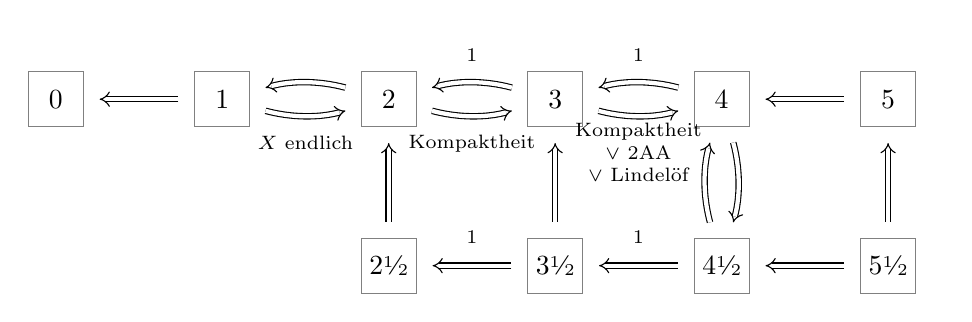
\begin{tikzpicture} [
			axiom/.style={rectangle,draw=black!50},
			node distance=14mm,
			minimum size=7mm,
			inner sep=1mm,
			implies/.style={double,-implies,double equal sign distance, shorten >=2mm, shorten <=2mm},
			label/.style={font=\scriptsize,auto,swap},
			bend angle=15,
		]
		\node[axiom] (T0) {\SepAxiom0};
		\node[axiom] (T1) [right=of T0] {\SepAxiom1};
		\node[axiom] (T2) [right=of T1] {\SepAxiom2};
		\node[axiom] (T3) [right=of T2] {\SepAxiom3};
		\node[axiom] (T4) [right=of T3] {\SepAxiom4};
		\node[axiom] (T5) [right=of T4] {\SepAxiom5};
		\node[axiom] (T2h) [below=of T2] {\SepAxiom{2\sfrac12}};
		\node[axiom] (T3h) [below=of T3] {\SepAxiom{3\sfrac12}};
		\node[axiom] (T4h) [below=of T4] {\SepAxiom{4\sfrac12}};
		\node[axiom] (T5h) [below=of T5] {\SepAxiom{5\sfrac12}};
		\draw[implies] (T1) to node[label] {} (T0);
		\draw[implies] (T2) to[bend right] node[label] {} (T1);
		\draw[implies] (T1) to[bend right] node[label] {$X$ endlich} (T2);
		\draw[implies] (T3) to[bend right] node[label] {\SepAxiom1} (T2);
		\draw[implies] (T2) to[bend right] node[label] {Kompaktheit} (T3);
		\draw[implies] (T4) to[bend right] node[label] {\SepAxiom1} (T3);
		\draw[implies] (T3) to[bend right] node[label,align=center] {Kompaktheit \\ $\lor$ 2AA \\ $\lor$ Lindelöf} (T4);
		\draw[implies] (T5) to node[label] {} (T4);
		\draw[implies] (T3h) to node[label] {\SepAxiom1} (T2h);
		\draw[implies] (T4h) to node[label] {\SepAxiom1} (T3h);
		\draw[implies] (T5h) to node[label] {} (T4h);
		\draw[implies] (T2h) to node[label] {} (T2);
		\draw[implies] (T3h) to node[label] {} (T3);
		\draw[implies] (T4h) to[bend left] node[label] {} (T4);
		\draw[implies] (T4) to[bend left] node[label] {} (T4h);
		\draw[implies] (T5h) to node[label] {} (T5);
	\end{tikzpicture}
	\caption{Zusammenhänge zwischen Trennungseigenschaften}
	\label{fig:separation_axioms}
\end{figure}

\begin{df}
	Ein topologischer Raum $(X, \scr T)$ heißt
	\begin{enumerate}[1)]
		\item
			\emph{hausdorffsch}, wenn $\SepAxiom2$ erfüllt ist,
		\item
			\emph{regulär}, wenn \SepAxiom1 und \SepAxiom3 erfüllt sind,
		\item
			\emph{vollständig regulär}, wenn \SepAxiom1 und \SepAxiom{3\sfrac 12} erfüllt sind,
		\item
			\emph{normal}, wenn \SepAxiom1 und \SepAxiom4 erfüllt sind,
		\item
			\emph{vollständig normal}, wenn \SepAxiom1 und \SepAxiom5 erfüllt sind,
		\item
			\emph{perfekt normal}, wenn \SepAxiom1 und \SepAxiom{5\sfrac 12} erfüllt sind.
	\end{enumerate}
\end{df}

\begin{lem}[Tychonoff]
	2AA und \SepAxiom3 impliziert \SepAxiom4.
\end{lem}

\begin{st}[Urysohn]
	Sei $(X, \scr T)$ ein \SepAxiom4-Raum.
	Dann gilt \SepAxiom{4\sfrac 12}.
	\begin{note}
		\SepAxiom4 besagt insbesondere:
		Zu $A \subset O$ mit $A$ abgeschlossen und $O$ offen existiert $U$ offen mit $A \subset U \subset  \_{U} \subset O$.
	\end{note}
	\begin{proof}
		Sei $A, B \subset X$ abgeschlossen, $A \cap B = \emptyset$.
		Setze $\_{A_0} = A_0 := B$, $A_1 := X \setminus A$.
		$A_1$ ist offene Umgebung von $\_{A_0}$.
		Sei $f_0: X \to [0,1]$ definiert durch $f_0|_{A_1} = 0, f_0|_{A} = 1$.
		Nach \SepAxiom4 existiert $A_{\f 12} \in \scr T$ mit
		\[
			B = \_{A_0} \subset A_{\f 12} \subset \_{A_{\f 12}} \subset A_1
		\]
		Sei $f: X \to [0,1], f|_{A_{\f 12}} = 0, f|_{A_1 \setminus A_{\f 12}} = \f 12, f|_A = 1$.

		Per Induktion erhalten wir $A_{\f {k}{2^n}} \in \scr T$ mit
		\[
			B = \_{A_{\f 0{2^n}}} \subset A_{\f 1{2^n}} \subset \_{A_{\f 1{2^n}}}
			\subset \dotsb \subset
			\_{A_{\f{2^n - 1}{2^n}}}
			\subset A_{\f {2^n}{2^n}}
			= X \setminus A.
		\]
		Wir definieren $f_n : X \to [0,1]$ durch $f|_{A_{\f 1{2^n}}} = 0$,
		\[
			f\Big|_{A_{\f {k+1}{2^n}} \setminus A_{\f {k}{2^n}}}
			= \f k{2^n}
		\]
		und $f|_A = 1$.
		Für jedes $x \in X$ ist $f_n(x) \in [0,1]$ monoton wachsend in $n$.
		Also $f_n(x) \to f(x) \in [0,1]$, $f_n$ konvergiert gleichmäßig gegen $f: X \to [0,1]$.

		Für $n \in \N$ wird $X$ überdeckt durch
		\begin{align*}
			U_n^0 &= A_{\f 1{2^n}} \\
			U_n^1 &= A_{\f 2{2^n}} \setminus A_{\f 0{2^n}} \\
			\vdots \quad &= \qquad \vdots \\
			U_n^{2^n-1} &= A_{\f {2^n}{2^n}} \setminus A_{\f {2^n-2}{2^n}} \\
			U_n^{2^n} &= X \setminus \_{A_{\f {2^n-1}{2^n}}}.
		\end{align*}
		Auf $U_n^k$ schwankt $f_n$ um höchstens $2^{-n}$ und $f$ um höchstens $2\cdot 2^{-n}$.
		Zu jedem $x \in X$ und $\eps > 0$ wählen wir $n \in \N$ so dass $2^{-n+1} < \eps$.
		Es gilt $x \in U_n^k$ für ein $k$.
		Dann ist
		\[
			f(U_n^k) \subset ]f(x) - \eps, f(x) + \eps[.
		\]
		Das bedeutet, $f$ ist stetig.
		% fixme: prüfen
	\end{proof}
\end{st}

\begin{lem}
	Sei $A \subset X$ abgeschlossen und $\phi: A \to [-s, s]$ stetig.
	Dann existiert $\Phi: X \to [-s, s]$ stetig mit
	\[
		|\phi(a) - \Phi(a)| \le \f 23 s
	\]
	für alle $a \in A$.
	\begin{proof}
		Setze $M := \phi^{-1}([-s, - \f s3]), N := \phi^{-1}([\f s3, s])$.
		$M, N$ sind ebgeschlossen.
		Nach Urysohn existiert $\Phi: X \to [-\f s3, \f s3]$ mit $\Phi|_M = - \f s3, \Phi|_N = \f s3$.
	\end{proof}
\end{lem}

\begin{st}[Tietze]
	Sei $(X, \scr T)$ ein \SepAxiom4-Raum.
	Ist $A \subset X$ abgeschlossen und $f: A \to [a,b]$ stetig.
	Dann existiert $F: X \to [a,b]$ stetig mit $F|_A = f$.
	\begin{proof}
		Sei \oBdA $[a,b] = [-1,1]$.
		Zu $f: A \to [-1,1]$ existiert $\Phi_0 : X \to [-\f 13, \f 13]$ wie im Lemma.
		Der Fehler auf $A$ ist $\phi_0 = f - \Phi_0|_A : A \to [-\f 23, \f 23]$.
		Zu $\phi_0$ existiert $\Phi_1: X \to [-\f 13 \cdot \f 23, \f 13 \cdot \f 23]$ wie im Lemma. % fixme: ref

		Per Induktion für $n \in \N$ ergibt sich der verbleibende Fehler als
		\[
			\phi_n = f - \Big( \Phi_0 + \Phi_1 + \dotsb + \Phi_n \Big)\Big|_A
			: A \to [-(\f 23)^{n+1}, (\f 23)^{n+1}.
		\]
		Dank Lemma existiert $\Phi_{n+1}: X \to [-\f 13(\f 23)^{n+1}, \f 13 (\f 23)^{n+1}]$.
		Damit konvergiert $F_n = \sum_{k=0}^n \Phi_n$ gleichmäßig auf $X$, denn
		\[
			\sum_{k=0}^n \|\Phi_k\|
			\le \sum_{k=0}^\infty \f 13 (\f 23)^k
			= 1.
		\]
		Die Grenzfunktion $F: X \to \R$ ist also stetig als glechimäßiger Grenzwert stetiger Funktionen und erfüllt
		\[
			\|F\| \le \sum_{k=0}^\infty \|\Phi_k\| = 1,
		\]
		also $F(X) \subset [-1, 1]$.
		Wegen $\phi_n \to 0$ gilt $f - F_n|_A \to 0$, also $F|_A = f$.
	\end{proof}
\end{st}

\begin{kor}
	Sei $(X, \scr T)$ ein \SepAxiom4-Raum.
	Ist $A \subset X$ abgeschlossen, $f: A \to \R^n$ stetig, so existiert $F: X \to \R^n$ stetig mit $F|_A = f$.
	\begin{note}
		Der Zielraum $\R^n$ ist wesentlich.
		Sei $Y = \R \setminus \{0\}, X = [-1,1], A = \{-1, 1\}, f: A \to Y, f(\pm 1) := \pm 1$.
		Hier existiert nach Zwischenwertsatz keine stetige Fortsetzung.
	\end{note}
\end{kor}

\begin{st}[Metrisierbarkeitssatz von Urysohn, 1924]
	Sei $(X, \scr T)$ ein topologischer Raum, der dem zweiten Abzählbarkeitsaxiom genügt.
	Dann sind äquivalent
	\begin{enumerate}[1)]
		\item
			$X$ ist metrisierbar,
		\item
			$X$ ist regulär, d.h. \SepAxiom1 und \SepAxiom3 ist erfüllt,
		\item
			$X$ ist normal, d.h. \SepAxiom1 und \SepAxiom4 ist erfüllt,
		\item
			$X$ ist homöomorph zu einem Teilraum von $[0,1]^\N$ (Hilbertwürfel).
	\end{enumerate}
	\begin{proof}
		\begin{segnb}[„(1)$\implies$(2)“]
			klar
		\end{segnb}
		\begin{segnb}[„(2)$\implies$(3)“]
			Folgt mit Lemma von Tychonoff. % fixme: ref
		\end{segnb}
		\begin{segnb}[„(3)$\implies$(4)“]
			Sei $\scr B$ eine abzählbare Basis.
			Sei $I$ die abzählbare Menge aller Paare $i = (U,V)$ mit $U,V \in \scr B$ und $\_U \subset V$.

			Dank Urysohn existiert $f_i: X \to [0,1]$ mit $f_i|_{\_U} = 0, f_i|_{X \setminus V} = 1$.
			Wir erhalten hieraus $h: X \to [0,1]^I, h(x) = (f_i(x))_{i \in I}$.
			Dies ist eine Einbettung.
		\end{segnb}
		\begin{segnb}[„(4)$\implies$(1)“]
			$[0,1]^\N$ ist metrisierbar, etwa durch
			\[
				d(x,y) = \sum_{k=0}^\infty 2^{-k-1} |x_i - y_i|,
			\]
			siehe Übungsaufgabe. % fixme: ref
		\end{segnb}
	\end{proof}
\end{st}

\chapter{Zusammenhang und Homotopie}

\coursetimestamp{26}{11}{2013}

\section{Zusammenhang}

\begin{st}
	Für jeden topologischen Raum $(X, \scr T)$ sind folgende Aussagen äquivalent:
	\begin{enumerate}[(1)]
		\item
			Jede stetige Funktion $f: X \to \R$ hat die Zwischenwerteigenschaft
		\item
			Für $f: X \to \R$ stetig ist $f(X) \subset \R$ ein Intervall.
		\item
			Jede stetige Funktion $f: X \to \{0,1\}$ (diskret) ist konstant.
		\item
			Jede stetige Funktion $f: X \to Y$ in einen diskreten Raum $Y$ ist konstant.
		\item
			Für jede offene Zerlegung $X = A \dunion B$ gilt $A = \emptyset$ oder $B = \emptyset$.
	\end{enumerate}
	$(X, \scr T)$ mit diesen Eigenschaften nennen wir \emph{zusammenhängend}.
	\begin{proof}
		\begin{segnb}[„$(1)\implies(2)\implies(3)$“]
			Leicht nachvollziehbar.
		\end{segnb}
		\begin{segnb}[„$(3)\implies(4)$“]
			Sei $x\in X, y := f(x)$ und $g: Y \to \{0,1\} \subset \R, g(y) := 1, g|_{Y\setminus \{y\}} := 0$.
			$g$ ist stetig, da $Y$ diskret, also konstant $g = 1$ nach Voraussetzung.
			Damit ist auch $f(X) \subset g^{-1}(1) = \{y\}$, also $f$ konstant.
		\end{segnb}
		\begin{segnb}[„$(4)\implies(5)$“]
			Sei $f : X \to \{0,1\}, f|_A := 0, f|_B := 1$.
			$f$ ist stetig (alle möglichen Urbilder sind offen in $X$), also ist $f$ nach Voraussetzung konstant und damit $A = f^{-1}(\{0\}) = \emptyset$ oder $B = f^{-1}(\{1\}) = \emptyset$.
		\end{segnb}
		\begin{segnb}[„$(5)\implies(1)$“]
			Sei $f: X \to \R$ stetig.
			Angenommen es existieren $y\in \R$ und $a,b \in X$ mit $f(a) \le y \le f(b)$, aber $y \not\in f(X)$.
			Dann wäre $X = A \dunion B$ mit $A = f^{-1}(\R_{<y}) \ni a, B = f^{-1}(\R_{>y}) \ni b$ eine offene Zerlegung von $X$, ein Widerspruch zur Voraussetzung.
		\end{segnb}
	\end{proof}
\end{st}

\begin{ex}
	\begin{itemize}
			%fixme: diskret, indiskret
		\item
			Jedes Intervall $I \subset \R$ ist zusammenhängend (ZWS).
		\item
			$\R \setminus \{a\}$ ist nicht zusammenhängen, denn $\R \setminus \{a\} = \R_{<a} \dunion \R_{>a}$.
		\item
			$\Q$ ist unzusammenhängend.
	\end{itemize}
\end{ex}

\begin{st}
	Sei $(X, <)$ linear geordnet.
	Jedes Intervall $I \subset X$ ist zusammenhängend genau dann, wenn $X$ vollständig geordnet und dicht ist.
	\begin{proof}
		Wie in $\R$, bzw. $\Q$.
	\end{proof}
\end{st}

\begin{proof}
	\begin{itemize}
		\item
			$(\R, <)$ ist vollständig geordnet, also $I \subset \R$ zusammenhängend.
		\item
			$(\Q, <)$ ist nicht vollständig geordnet.
			Das Intervall $[0,1]_\Q$ ist nicht zusammenhängend, denn für $\xi \in [0,1] \setminus [0,1]_\Q$ ist
			\[
				[0,1]_\Q =
				\Set{ x \in \Q | 0 \le x < \xi }
				\dunion
				\Set{ x \in \Q | \xi < x \le 1 }
			\]
			eine offene Zerlegung.
	\end{itemize}
\end{proof}

\begin{st}
	Ist $f: X \to Y$ stetig und $X$ zusammenhängend, so auch $f(X)$.
	\begin{proof}
		Ist $f(X) = A \dunion B$ offene Zerlegung, so auch $X = f^{-1}(A) \dunion f^{-1}(B)$, also $A = \emptyset$ oder $B = \emptyset$.
	\end{proof}
\end{st}

\begin{lem}
	Sei $X$ ein topologischer Raum und $A_i \subset X$ für $i \in I$ zusammenhängend.
	Für jedes Paar $i,j \in I$ existiere eine Kette $i = i_0 , i_1, \dotsc, i_n = j$ in $I$ mit $A_{i_{k-1}} \cap A_{i_k} \neq \emptyset$ für $k = 1, \dotsc, n$.

	Dann ist $A = \bigcup_{i\in I} A_i$ zusammenhängend.
	\begin{proof}
		Sei $f: A \to \{0,1\}$ stetig.
		Dann ist $f_i := f|_{A_i}: A_i \to \{0,1\}$ stetig, also $f_i$ konstant, kurz $f_i = c_i$.
		Für $i = i_0, \dotsc, i_n = j$ wie oben gilt dann $c_i = \dotsb = c_j$.
	\end{proof}
\end{lem}

\begin{lem}
	Seien $X_1, \dotsc, X_n$ zusammenhängend, so auch $X = X_1 \times \dotsb \times X_n$.
	\begin{proof}
		Sei $a \in X$ und $f: X \to \{0,1\}$ stetig.
		Zu $b \in X$ betrachte
		\begin{align*}
			A_i &= \{ b_1 \} \times \dotsb \times \{b_{i-1}\} \times X_i \times \{a_{i+1}\} \times \dotsb \times \{a_n\} \\
			&\homeomorphic X_i.
		\end{align*}
		Es gilt $a \in A_1$, $b \in A_n$ und $A_{i-1} \cap A_i \ni (b_1, \dotsc, b_{i-1}, a_i, \dotsc, a_n)$.
		Nach dem Lemma ist $A_1 \cup \dotsb \cup A_n$ zusammenhängend, also $f(b) = f(a) = \const$.
	\end{proof}
\end{lem}

\begin{lem}
	Sei $(X, \scr T)$ ein topologischer Raum, $A \subset X$ zusammenhängend und $A \subset B \subset \_A$.
	Dann ist auch $B$ zusammenhängend.
	\begin{proof}
		Sei $f: B \to \{0,1\}$ stetig, dann ist $f|_A = c$ konstant.
		Die Abbildungen $f, c: B \to \{0,1\}$ sind stetig und stimmen auf $A$ überein.
		$A$ ist dicht in $B$ und $\{0,1\}$ ist hausdorffsch.
		Also gilt $f=c$.
	\end{proof}
\end{lem}

\begin{st}
	Sei $(X_i)_{i\in I}$ eine Familie topologischer Räume mit $X_i \neq \emptyset$.
	Der Produktraum $X = \prod_{i\in I} X_i$ ist genau dann zusammenhängend, wenn jedes $X_i$ zusammenhängend ist.
	\begin{proof}
		\begin{segnb}[„$\implies$“]
			Klar, da $p_i: X \to X_i$ stetig und surjektiv ist.
		\end{segnb}
		\begin{segnb}[„$\implies$“]
			Sei $a \in X$.
			Für $J \subset I$ endlich sei
			\begin{align*}
				A_J &:= \prod_{i\in I} A_i, &
				A_j &:= \begin{cases}
					X_j & j \in J \\
					\{a_j\} & j \in I \setminus J
				\end{cases}.
			\end{align*}
			$A_j$ ist zusammenhängend nach obigem Lemma.
			Damit ist auch $A = \bigcup_{J} A_J$ zusammenhängend, denn $A_J \cap A_j \ni \{a\}$.

			Es gilt außerdem $\_A = X$:
			Jede offen Menge $U \subset X$ enthält $\prod_{i \in I} U_i$, wobei $U_i \subset X_i$ offen und $U_i = X_i$ für $i \in I \setminus J$ außerhalb einer endlichen Menge.
			Ist $U$ nicht-leer, dann gilt $U_i \neq \emptyset$ für alle $i \in I$.
			Demnach existiert $b \in U$ mit $b_j \in U_j$ für alle $j \in J$ und $b_i = a_i$ für alle $i \in I \setminus j$.
			Damit gilt $b \in A_J$, also $b \in U \cap A$.
		\end{segnb}
	\end{proof}
\end{st}

%fixme \eqq ===
\begin{df}
	Sei $(X, \scr T)$ ein topologischer Raum.
	Für $x,y \in X$ definieren wir $x \eqq y$ durch die Bedingung, dass $x,y$ in einer zusammenhängenden Teilmenge von $X$ liegen.
	Dies ist eine Äquivalenzrelation.
	Die Äquivalenzklasse $\scr Z(x)$ von $x$ heißt \emph{(Zusammenhangs-)Komponente} von $x$ in $X$.
	Die definiert die Zerlegung
	\[
		\scr Z(X) := \{ \scr Z(x) : x \in X \}.
	\]
\end{df}

\begin{ex}
	\begin{itemize}
		\item
			$X$ ist zusammenhängend genau dann, wenn $\scr Z(X) = \{X\}$.
		\item
			$\scr Z(\R \setminus \{0\}) = \{ \R_{<0}, \R_{>0} \}$.
		\item
			$\scr Z(\Q) = \{ \{x\} : x \in \Q \}$.
	\end{itemize}
\end{ex}

\begin{st}
	\begin{enumerate}[(1)]
		\item
			$\scr Z(x)$ ist der größte zusammenhängende Teilraum von $X$, der $x$ enthält.
		\item
			Jede Komponente $\scr Z(x)$ ist abgeschlossen.
		\item
			Ist die Zerlegung $\scr Z(X)$ endlich, so ist jede Komponente offen und $X = \bigdunion \scr Z(X)$ ist eine Summentopologie.
	\end{enumerate}
\end{st}

\begin{st}
	\begin{enumerate}[(1)]
		\item
			Ist $f: X \to Y$ stetig, so gilt $f(\scr Z(x)) \subset \scr Z(f(x))$.
		\item
			Wir erhalten hieraus $\scr Z(f): \scr Z(X) \to \scr Z(Y): \scr Z(x) \mapsto \scr Z(f(x))$.
		\item
			Es gilt $\scr Z(\Id_X) = \Id_{\scr Z(X)}$ und $\scr Z(g\circ f) = \scr Z(g) \circ \scr Z(f)$.
	\end{enumerate}
	\begin{proof}
		(1) und (2) sind klar nach den vorigen Ergebnissen, zeige noch (3).
		Es gilt
		\begin{align*}
			\scr Z(g\circ f) (\scr Z(x))
			&= \scr Z(g(f(\scr Z(x)))) \\
			&= \scr Z(g) (\scr Z(f(\scr Z(x)))) \\
			&= \scr Z(g)(\scr Z(f)(\scr Z(x))) \\
			&= (\scr Z(g) \circ \scr Z(f)) (\scr Z(x)).
		\end{align*}
	\end{proof}
\end{st}


\section{Wegzusammenhang}

Analog zum Weg in metrischen Räumen definieren wir Wege in topologischen Räumen.

\begin{df}
	Ein \emph{Weg} im topologischen Raum $(X, \scr T)$ ist eine stetige Abbildung $\gamma: [0,1] \to X$.
	Dabei heißt $\gamma(0) = a$ \emph{Anfangspunkt} und $\gamma(1) = b$ \emph{Endpunkt}.

	Der Raum $X$ heißt \emph{wegzusammenhängend}, wenn zu jedem Paar $a,b \in X$ ein Weg von $a$ nach $b$ in $X$ existiert (d.h. $\gamma:[0,1] \to X$ stetig mit $\gamma(0) = a, \gamma(1) = b$).

	Wir definieren die Menge aller Wege $P(X)$ und die Menge aller Wege von $a$ nach $b$, $P(X, a, b)$ als
	\begin{align*}
		P(X) &= \scr C ([0,1], X), \\
		P(X, a, b) &= \{ \gamma : [0,1] \to X \text{ stetig } : \gamma(0) = a, \gamma(1) = b \}.
	\end{align*}
	Außerdem folgende Abbildungen, bzw. Operatoren:
	\begin{enumerate}[1)]
		\item
			$X \injto P(X), a \mapsto \const_{[0,1]}^a$,
		\item
			$\_\  : P(X, a, b) \to P(X, b, a), \_\gamma(t) := \gamma(1-t)$,
		\item
			$\ast: P(X, a, b) \times P(X, b, c) \to P(X, a, c)$ durch
			\[
				(\gamma_1 \ast \gamma_2)(t) := \begin{cases}
					\gamma_1 (2t) & 0 \le t \le \f 12 \\
					\gamma_2 (2t - 1) & \f 12 \le t \le 1
				\end{cases}.
			\]
	\end{enumerate}
\end{df}

\begin{df}
	Wir nennen $x,y \in X$ \emph{verbindbar} in $X$ (durch einen Weg in $X$), wenn ein Weg $\gamma: [0,1] \to X$ von $\gamma(0) = x$ nach $\gamma(1) = y$ existiert.
	Dies ist eine Äquivalenzrelation.

	Die Äquivalenzklasse $[x]$ von $x$ heißt \emph{Weg(-zusammenhangs)komponente}.
	Dies definiert die Zerlegung
	\[
		\pi_0 (X) := \{ [x] : x \in X \}.
	\]
	$X$ heißt \emph{wegzusammenhängend}, wenn $\pi_0(X) = \{X\}$.
\end{df}

\begin{ex}
	\begin{itemize}
		\item
			Jedes Intervall $I \subset \R$ ist wegzusammenhängend.
		\item
			Jede sternförmige Menge $X \subset \R^n$ ist wegzusammenhängend.
		\item
			$\S^n \subset \R^{n+1}$ ist wegzusammenhängend für $n \ge 1$.
	\end{itemize}
\end{ex}

\begin{st}
	Wegzusammenhang impliziert Zusammenhang, aber nicht umgekehrt.
	\begin{proof}
		Wie im metrischen Fall.
		Gegenbeispiel folgt. % fixme: ref
	\end{proof}
\end{st}

\begin{ex}
	Sei
	\begin{align*}
		A &:= \Set{ (x, \sin( \f {\pi}x)) | x \in ]0,1] } \\
		B &:= \{0\} \times [-1, 1]
	\end{align*}
	$C = \_A = A \cup B$ ist zusammenhängend, aber nicht wegzusammenhängend.
\end{ex}

\coursetimestamp{02}{12}{2013}

\begin{st}
	Ist $f: X \to Y$ stetig und $X$ wegzusammenhängend, so auch $f(X)$.
\end{st}

\begin{st}
	Seien $(X_i, \scr T_i)$ mit $X_i \neq \emptyset$ topologische Räume.
	Genau dann ist $\prod_{i \in I} X_i$ wegzusammenhängend, wenn jeder Raum $X_i$ dies ist.
	\begin{proof}
		Folgt mit universeller Abbildungseigenschaft und dem letzten Satz.
	\end{proof}
\end{st}

\begin{st}
	\begin{enumerate}[1)]
		\item
			Ist $f: X \to Y$ stetig, so gilt
			\[
				f([a]_X) \subset [f(a)]_Y.
			\]
		\item
			Wir erhalten mit 1) die Abbildung \\ $\pi_0(f): \pi_0(X) \to \pi_0(Y): [a]_X \mapsto [f(a)]_Y$.
		\item
			Es gilt $\pi_0(\Id_X) = \Id_{\pi_0(X)}$ und $\pi_0(g \circ f) = \pi_0(g) \circ \pi_0(f)$.
			Das folgende Diagramm kommutiert:
			\[
				\begin{tikzcd}[row sep=small]
					X \arrow{dr}{f} \arrow{dd}[left]{g\circ f} \arrow{rr} &  & \pi_0(X) \arrow{dr}{\pi_0(f)} & \\
					& Y \arrow{dl}{g} \arrow{rr} &  & \pi_0(Y) \arrow{dl}{\pi_0(g)}\\
					Z \arrow{rr}  & & \pi_0(Z) \arrow[leftarrow, crossing over]{uu}[yshift=5mm]{\pi_0(g\circ f)} &
				\end{tikzcd}.
			\]
	\end{enumerate}
	\begin{proof}
		\begin{enumerate}[1),start=3]
			\item
				Es gilt
				\begin{align*}
					\pi_0(g\circ f)([a]_X)
					&= [(g\circ f)(a)]_Z
					= [g(f(a))]_Z
					= \pi_0(g)([f(a)]_Y) \\
					&= \pi_0(g)(\pi_0(f)([a]_X))
					= (\pi_0(g)\circ \pi_0(f))([a]_X).
				\end{align*}
		\end{enumerate}
	\end{proof}
\end{st}


\section{Lokaler Zusammenhang}


\begin{df}
	Ein topologischer Raum $(X, \scr T)$ heißt \emph{lokal (weg-)zusammenhängend} in $a \in X$, wenn jede offene Umgebung von $a$ in $X$ eine (weg-)zusammenhängende offene Umgebung enthält.
\end{df}

\begin{ex}
	\begin{itemize}
		\item
			$\R^n$ ist lokal wegzusammenhängend, denn $B(a,\eps)$ ist sternförmig und somit wegzusammenhängend.
			Ebenso jeder topologische Vektorraum (ausgeglichene Umgebung ist sternförmig).
		\item
			Ist $X$ lokal wegzusammenhängend, so auch jede offene Teilmenge $U \subset X$.
	\end{itemize}
\end{ex}

\begin{ex}
	\begin{itemize}
		\item
			Die „Sinuskurve des Topologen“ % fixme: ref
			ist zusammenhängend, aber nicht lokal zusammenhängend.
		\item
			Der „rationale Kamm“
			\[
				X = ([0,1] \times \{0\}) \cup ([0,1]_\Q \times [0,1])
			\]
			ist wegzusammenhängend, aber nicht lokal wegzusammenhängend.
		\item
			$X = [0,1] \cup [2,3]$ ist lokal (weg-)zusammenhängend, aber nicht global (weg-)zusammenhängend.
	\end{itemize}
\end{ex}

Zu jedem Raum $X$ haben wir die Zerlegungen $X = \bigdunion \scr Z(X)$ und $X = \bigdunion \pi_0(X)$.

\begin{st}
	Ist $X$ lokal zusammenhängend, so ist die Zerlegung $X = \bigdunion \scr Z(X)$ offen.

	Ist $X$ lokal wegzusammenhängend, so ist die Zerlegung $X = \bigdunion \pi_0(X)$ offen.
	In diesem Fall gilt $\pi_0(X) = \scr Z(X)$.
	\begin{proof}
		Leicht nachzuvollziehen.
	\end{proof}
\end{st}


\section{Homotopie stetiger Abbildungen}


\begin{df}
	Eine \emph{Homotopie} ist eine stetige Abbildung $H: [0,1] \times X \to Y$.
	Für jedes $t \in [0,1]$ ist dann $H_t: X \to Y$ mit $H_t(x) := H(t,x)$ stetig.

	Zwei stetige Abbildungen $f,g : X \to Y$ heißen \emph{homotop} in $Y$, wenn es eine Homotopie $H: [0,1] \times X \to Y$ mit $H_0 = f$ und $H_1 = g$ gibt.
	Wir schreiben dann $H: f \homotopic g$, oder $f\homotopic g$

	Ist $f: X \to  Y$ homotop zu $\const_X^{\{\ast\}}: X \to \{\ast\} \subset Y$, so nennen wir $f$ \emph{nullhomotop}, Kurz $f \homotopic \ast$.
	Der Raum $X$ heißt \emph{zusammenziehbar}, wenn $\Id_X \homotopic \ast$.
\end{df}

\begin{ex}
	Sei $X \subset \R^n$ sternförmig bezüglich $a \in X$ (z.B. $X = \R^n, a = 0$).

	Dann ist $X$ zusammenziehbar mittels $H: [0,1] \times X \to X, H(t,x) = (1-t)x + ta$.

	Es gilt $H_0 = \Id_X, H_1 = \const_X^{a}$.
	$H$ ist wohldefiniert und stetig für alle $(t,x) \in [0,1] \times X$.
\end{ex}

\begin{st}
	Seien $f,g : X \to \S^n$ stetig und nirgends antipodal, d.h. $f(x) \neq -g(x)$ für alle $x \in X$.
	Dann sind $f$ und $g$ homotop in $\S^n$ mittels
	\[
		H(t,x) := \f {(1-t)f(x) - tg(x)}{|(1-t)f(x) - tg(x)|}.
	\]
	\begin{proof}
		klar
	\end{proof}
\end{st}

\begin{kor}
	Ist $f: X \to \S^n$ stetig, aber nicht surjektiv, so gilt $f \homotopic *$.
	\begin{proof}
		Es gibt zwei Möglichkeiten, dies zu beweisen:
		\begin{enumerate}[1.]
			\item
				Wähle $a \in \S^n \setminus (X)$ und $g = \const_X^{-a}$, dann ist $f \homotopic g$ wie im letzten Satz.
			\item
				Mittels stereographischer Projektion.
				Für $a \in \S^n \setminus f(X)$ ist $\S^n \setminus \{a\} \homeomorphic \R^n \homotopic *$ wie im Beispiel.
		\end{enumerate}
	\end{proof}
\end{kor}

\begin{df}
	\begin{enumerate}[(1)]
		\item
			Zu $f: X \to Y$ haben wir $H: f \homotopic f$ mit $H(t,x) = f(x)$.
		\item
			Zu $H: f \homotopic g$ definieren wir $\_H: g \homotopic f$ mit $H(t,x) := H(1-t,x)$.
		\item
			Zu $H: f \homotopic g$ und $K: g\homotopic h$ definieren wir $(H \ast K) : f \homotopic h$ durch
			\[
				(H \ast K)(t,x) = \begin{cases}
					H(2t, x) & 0 \le t \le \f 12 \\
					K(2t-1), x) & \f 12 \le t \le 1
				\end{cases}.
			\]
	\end{enumerate}
	Homotopie ist eine Äquivalenzrelation.
\end{df}

\begin{df}
	Die Menge der Homotopieklassen von $\scr C(X, Y)$ bezeichnen wir mit
	\[
		[X,Y] := \scr C(X, Y) / \homotopic.
	\]
\end{df}

%fixme : anmerkung zur notation
\begin{st}
	Aus $H: f_0 \homotopic f_1 : X \to Y$ und $K: g_0 \homotopic g_1: Y \to Z$ folgt $L: g_0 \circ f_0 \homotopic g_1 \circ f_1$ mittels
	\[
		L(t, x) = K(t, H(t,x)).
	\]
	Wir schreiben auch $L_t = K_t \circ H_t$.
\end{st}

\begin{kor}
	Wir haben eine Kategorie \emph{Toph}:
	\begin{itemize}
		\item
			Objekte sind topologische Räume $X, Y, Z, \dotsc $,
		\item
			Morphismen sind Homotopieklassen $[f]$ von stetigen Abbildungen $f: X \to Y$,
		\item
			Die Komposition ist $[g] \circ [f] = [g\circ f]$.
	\end{itemize}
\end{kor}

\begin{st}
	Der Funktor $\pi_0: \mathrm{Top} \to \mathrm{Set}$ ist homotopie-invariant, d.h. aus $f \homotopic g$ folgt $\pi_0(f) = \pi_0(g)$.
	\[
		\begin{tikzcd}[row sep=tiny]
			\mathrm{Top} \arrow{dr}{\pi_0} \arrow{dd}[left]{q} & \\
			& \mathrm{Set} \\
			\mathrm{Toph} \arrow{ur}[below]{\pi_0} & \\
		\end{tikzcd}.
	\]
\end{st}

\begin{df}
	Zwei Räume $X, Y$ heißen \emph{homotopie-äquivalent}, geschrieben $X \homotopic Y$, wenn es stetige Abbildungen $f: X \to Y$ und $g: Y \to X$ gibt mit $g \circ f \homotopic \Id_X$ und $f \circ g \homotopic \Id_Y$.
\end{df}

\begin{ex}
	\begin{enumerate}[1)]
		\item
			Falls $X \homeomorphic Y$, dann auch $X \homotopic Y$.
		\item
			Aus $X \homotopic Y$ folgt nicht $X \homeomorphic Y$, z.b. $\R \not \homeomorphic \R^2$, aber $\R \homotopic \R^2 \homotopic \ast$.
	\end{enumerate}
\end{ex}

\begin{ex}
	$X = \S^n$ und $Y = \R^{n+1} \setminus \{0\}$ sind homotopie-äquivalent.
	\begin{proof}
		Sei $f: X \injto Y$ die Inklusion und $g: Y \to X, g(y) = \f y{|y|}$.
		Es gilt $g \circ f = \Id_X$ ($g$ ist \emph{Retrakt}) und $f \circ g \homotopic \Id_Y$ mittels
		\[
			H(t,y) = ty + (1-t) g(y) \in Y.
		\]
		$H$ ist \emph{(starker) Deformationsretrakt}.
	\end{proof}
\end{ex}




\chapter{Die Sprache der Kategorien}

\coursetimestamp{03}{12}{2013}


\section{Kategorien}


\begin{df}
	Eine \emph{Kategorie} $\Cat C = (\Ob, \Mor, \circ)$ besteht aus
	\begin{enumerate}[a)]
		\item
			Eine Klasse $\Ob$ von \emph{Objekten} $A, B, C, D, \dotsc \in \Ob$
		\item
			zu je zwei Objekten $A, B \in \Ob$ eine Klasse $\Mor(A,B)$ von \emph{Morphismen} von $A$ nach $B$,
		\item
			zu $A, B, C \in \Ob$ eine \emph{Verknüpfung}
			\[
				\circ: \Mor(B, C) \times \Mor(A, B) \to \Mor(A, C).
			\]
	\end{enumerate}
	Diese solllen folgenden Bedingungen genügen:
	\begin{enumerate}[1)]
		\item
			Zu jedem $B \in \Ob$ existiert $\Id_B \in \Mor(B, B)$, sodass $\Id_B \circ f = f$ und $g \circ \Id_B = g$ für alle $A, C \in \Ob$ und $f \in \Mor(A, B)$ und $g \in \Mor(B, C)$.
		\item
			Es gilt Assoziativität: $h \circ (g \circ f) = (h \circ g) \circ f$ für alle $A, B, C, D \in \Ob$ und $f \in \Mor(A, B), g \in \Mor(B, C), h \in \Mor(C, D)$.
	\end{enumerate}
\end{df}

\begin{ex}
	\begin{itemize}
		\item
			$\Cat{Top}$: (topologische Räume, stetige Abbildungen, Komposition)
		\item
			$\Cat{Set}$: (Mengen, Abbildungen, Komposition).
			Auch mit nur injektiven oder nur surjektiven Abbildungen bildet $\Cat{Set}$ eine Kategorie.
		\item
			$\Cat{FinSet}$: (endliche Mengen, Abbildungen, Komposition)
		\item
			$(X, \le, \text{Transitivität})$
		\item
			$\Cat{Grp}$: (Gruppen, Gruppenhomomorphismen, Komposition)
		\item
			$\Cat{FinGrp}$: (endliche Gruppen, Gruppenhomomorphismen, Komposition)
		\item
			$\Cat{Ab}$: (abelsche Gruppen, Gruppenhomomorphismen, Komposition)
		\item
			$\Cat{\Vec_K}$: ($K$-Vektorräume, $K$-lineare Abbildungen, Komposition)
		\item
			$\Cat{\Mat_K}$: ($\N$, Matrizen über $K$, Multiplikation)
			\[
				\Mat_K(q,r) \times \Mat(p,q) \to \Mat_K(p,r)
			\]
	\end{itemize}
\end{ex}

\paragraph{Kommutative Diagramme}

Ein Diagramm
\[
	\begin{tikzcd}[column sep=small]
		& B \arrow{dr}{g} & \\
		A \arrow{ur}{f} \arrow{rr}{h} & & C
	\end{tikzcd}
\]
kommutiert, falls $h = g \circ f$.

\begin{ex}
	\begin{itemize}
		\item
			\[
				\begin{tikzcd}[row sep=tiny]
					& B \arrow{dr}{g} \arrow{dd}{\Id_B} & \\
					A \arrow{ur}{f} \arrow{dr}[below]{f} & & C \\
					& B \arrow{ur}[below]{g} &
				\end{tikzcd}
			\]
		\item
			\[
				\begin{tikzcd}[column sep=large]
					~& B \arrow{dr}{h\circ g} & \\
					A \arrow{ur}{f} \arrow{rr}[xshift=-7mm]{(h\circ g) \circ f}\arrow{rr}[xshift=-7mm,swap]{h\circ (g \circ f)} \arrow{dr}[swap]{g\circ f} & & D \\
					& C \arrow[leftarrow,crossing over]{uu}[yshift=5mm,swap]{g} \arrow{ur}[swap]{h} &
				\end{tikzcd}
			\]
		\item
			$g$ ist Linksinverse von $f$; $g$ ist Rechtsinverse von $f$; $f$ und $g$ sind zueinander invers:
			\[
				\begin{tikzcd}
					X \arrow{d}[swap]{\Id_X} \arrow{r}{f} & Y \arrow{dl}{g} \\
					X &
				\end{tikzcd}
				\!
				\begin{tikzcd}
					~& Y \arrow{d}{\Id_Y} \arrow{dl}[swap]{g} \\
					X \arrow{r}{f} & Y
				\end{tikzcd}
				\qquad
				\begin{tikzcd}
					X \arrow{r}{f} \arrow{d}[left]{\Id_X} & Y \arrow{d}{\Id_Y} \arrow{dl}{g} \\
					X \arrow{r}[below]{f} & Y
				\end{tikzcd}
			\]
	\end{itemize}
\end{ex}

\begin{df}
	\begin{itemize}
		\item
			Zwei Morphismen $f: X \to Y$ und $g: Y \to X$ in $\Cat{C}$ heißen \emph{zueinander invers}, wenn $g \circ f = \Id_X$ und $f \circ g = \Id_Y$ gilt.
		\item
			Wir nennen $f: X \to Y$ in $\Cat{C}$ invertierbar, oder einen $\Cat{C}$-Isomorphismus, geschrieben $f: X \isoto Y$, wenn es zu $f$ in $\Cat{C}$ einen inversen Morphismun $g: Y \to X$ gibt.
		\item
			Zwei Objekte $X, Y \in \Cat{C}$ heißen \emph{isomorph}, geschrieben $X \isomorphic Y$, wenn ein Isomorphismus $f: X \to Y$ existiert.
	\end{itemize}
\end{df}

\begin{ex}
	\begin{itemize}
		\item
			In $\Cat{Set}$ sind Bijektionen Isomorphismen.
		\item
			In $(X, \le, \text{Transitivität})$ bedeutet Isomorphie Gleichheit.
		\item
			In $\Cat{\Vec_K}$ $K$-lineare Isomorphismen.
		\item
			In $\Cat{\Mat_K}$ beudetet Isomorphie $m = n$ in $\N$.
		\item
			In $\Cat{Grp}$ Gruppenisomorphismen.
		\item
			In $\Cat{Top}$ Homöomorphismen.
	\end{itemize}
\end{ex}


\section{Funktoren}


\begin{df}
	Seien $\Cat{C}, \Cat{D}$ Kategorien.
	Ein \emph{kovarianter Funktor} $F: \Cat{C} \to \Cat{D}$ ordnet jedem Objekt $X$ in $\Cat{C}$ ein Objekt $F(X)$ in $\Cat{D}$ zu und jedem Morphismus $f: X \to Y$ in $\Cat{C}$ einen Morphismus $F(f) : F(X) \to F(Y)$ in $\Cat{D}$, sodass $F(\Id_X) = \Id_{F(X)}$ und $F(g\circ f) = F(g) \circ F(f)$.
	\[
		\begin{tikzcd}[column sep=small]
			~ & Y \arrow{dr}{g} & \\
			X \arrow{ur}{f} \arrow{rr}[swap]{h} & & Z
		\end{tikzcd}
		\mapsto
		\begin{tikzcd}[column sep=tiny]
			~ & F(Y) \arrow{dr}{F(g)} & \\
			F(X) \arrow{ur}{F(f)} \arrow{rr}[swap]{F(h)} & & F(Z)
		\end{tikzcd}
	\]
\end{df}

\begin{ex}
	\begin{itemize}
		\item
			\emph{kontravarianter Funktor}:
			\begin{align*}
				\Hom_K(\argdot, K): \Vec_K &\to \Vec \\
				V &\mapsto V^* = \Hom_K(V,K) \\
				(f: V \to W) &\mapsto (f^*: W^* \to V^*, f^*(h) = h \circ f)
			\end{align*}
		\item
			\emph{kovarianter Funktor}:
			\begin{align*}
				\Hom_K(X, \argdot) : \Vec_K &\to \Vec_K \\
				V & \mapsto \Hom_K(X, V) \\
				(f: V \to W) & \mapsto (f_*: \Hom(X, V) \to \Hom(X, V), f_*(h) = f \circ h)
			\end{align*}
	\end{itemize}
\end{ex}

\begin{df}
	Ein \emph{kontravarianter Funktor} $G: \Cat{C} \to \Cat{D}$ ordnet jedem Objekt $X$ in $\Cat{C}$ ein Objekt $G(X)$ in $\Cat{D}$ zu und jedem Morphismus $f: X \to Y$ in $\Cat{C}$ einen Morphismus $G(f) : G(Y) \to G(X)$ in $\Cat{D}$, sodass $G(\Id_X) = \Id_{G(X)}$ und $G(g\circ f) = G(f) \circ G(g)$
	\[
		\begin{tikzcd}[column sep=small]
			~ & Y \arrow{dr}{g} & \\
			X \arrow{ur}{f} \arrow{rr}{h} & & Z
		\end{tikzcd}
		\mapsto
		\begin{tikzcd}[column sep=tiny]
			~ & G(Y) \arrow[leftarrow]{dr}{G(g)} & \\
			G(X) \arrow[leftarrow]{ur}{G(f)} \arrow[leftarrow]{rr}{G(h)} & & G(Z)
		\end{tikzcd}
	\]
\end{df}

\begin{ex}
	\begin{itemize}
		\item
			Zusammenhangskomponenten
			\begin{align*}
				\scr Z: \Cat{Top} &\to \Cat{Set} \\
				X &\mapsto \scr Z(X) \\
				(f:X \to Y) &\mapsto (\scr Z(f): \scr Z(X) \to \scr Z(Y))
			\end{align*}
		\item
			Wegzusammenhangskomponenten
			\begin{align*}
				\pi_0: \Cat{Top} &\to \Cat{Set} \\
				X & \mapsto \pi_0(X) \\
				(f: X \to Y) &\mapsto (\pi_0(f): \pi_0(X) \to \pi_0(Y))
			\end{align*}
		\item
			„Vergiss“-Funktor (die Topologie wird „vergessen“)
			\begin{align*}
				V: \Cat{Top} &\to \Cat{Set} \\
				(X,\scr T) & \mapsto X \\
				(f: (X,\scr T_X) \to (Y, \scr T_Y)) &\mapsto (f: X \to Y)
			\end{align*}
		\item
			Potenzmenge (kovariant)
			\begin{align*}
				\scr P_*: \Cat{Set} & \to \Cat{Set} \\
				X, & \mapsto \scr P(X) \\
				(f: X \to Y) &\mapsto (f_*: \scr P(X) \to \scr P(y), f_*(A) := f(A))
			\end{align*}
		\item
			Potenzmenge (kontravariant)
			\begin{align*}
				\scr P^*: \Cat{Set} & \to \Cat{Set} \\
				X & \mapsto \scr P(X) \\
				(f: X \to Y) &\mapsto (f^*: \scr P(Y) \to \scr P(X), f^*(B) := f^{-1}(B))
			\end{align*}
	\end{itemize}
\end{ex}


\section{Transformationen}


\begin{df}
	Seien $F, G: \Cat{C} \to \Cat{D}$ Funktoren.
	Eine \emph{(natürliche) Transformation} $t: F \to G$ ordnet jedem Objekt $X$ in $\Cat{C}$ einen Morphismus $t(X): F(X) \to G(X)$ in $\Cat{D}$ zu, sodass für jeden Morphismus $f: X \to Y$ in $\Cat{C}$ die Gleichung $t(Y) \circ F(f) = G(f) \circ t(X)$ gilt.
	\[
		\begin{tikzcd}
			X \arrow{d}{f} & F(X) \arrow{d}{F(f)} \arrow{r}{t(X)} & G(X) \arrow{d}{G(f)} \\
			Y & F(Y) \arrow{r}{t(Y)} & G(Y)
		\end{tikzcd}
	\]
	Gilt hierbei $t(X) : F(X) \isoto G(X)$ für alle $X$, so heißt $t$ \emph{(natürliche) Äquivalenz} von $F$ und $G$.
\end{df}

\begin{ex}
	\[
		\begin{tikzcd}
			~ & \pi_0(X) \arrow{dd}[yshift=5mm]{t(X)} \arrow{rr}{\pi_0} & & \pi_0(Y) \arrow{dd}{t(Y)} \\
			X \arrow{ur}{a\mapsto [a]_X} \arrow{dr}[swap]{a\mapsto \scr Z_X(a)} \arrow[crossing over]{rr}[swap,xshift=5mm]{f} & & Y \arrow{ru}{b\mapsto[b]_Y} \arrow{dr}[swap]{b\mapsto \scr Z_Y(b)} & \\
			& \scr Z(X) \arrow{rr}[below]{\scr Z(f)} && \scr Z(Y)
		\end{tikzcd}
%		\begin{tikzcd}[row sep=small,column sep=small]
%			X \arrow{dr}{f} \arrow{dd}[left]{g\circ f} \arrow{rr} &  & \pi_0(X) \arrow{dr}{\pi_0(f)} & \\
%			& Y \arrow{dl}{g} \arrow{rr} &  & \pi_0(Y) \arrow{dl}{\pi_0(g)}\\
%			Z \arrow{rr}  & & \pi_0(Z) \arrow[leftarrow, crossing over]{uu}[yshift=5mm]{\pi_0(g\circ f)} &
%		\end{tikzcd}.
	\]
	mit
	\begin{align*}
		t(X): \pi_0(X) &\to \scr Z(X) \\
		[a]_X &\mapsto \scr Z_X(a)
	\end{align*}
	\begin{note}
		Lokale wegzusammenhängende Räume bilden eine Unterkategorie von $\Cat{Top}$.
		Hierauf sind die Funktoren $\pi_0$ und $\scr Z$ natürlich äquivalent.
	\end{note}
\end{ex}





\end{document}
